\documentclass[11pt]{article}
\usepackage{geometry}
\usepackage{graphicx}
\usepackage{wrapfig}
\usepackage{float}
\usepackage{caption}
\usepackage{subcaption}
\usepackage[T1]{fontenc}
\usepackage[utf8]{inputenc}
\usepackage{helvet}
\renewcommand{\familydefault}{\sfdefault}
%\usepackage{titlesec}
%\titlespacing\section{1pt}{12pt plus 2pt minus 2pt}{1pt plus 2pt minus 2pt}
%\titlespacing\subsection{1pt}{12pt plus 2pt minus 2pt}{pt plus 2pt minus 2pt}
%\titlespacing\subsubsection{5pt}{12pt plus 2pt minus 2pt}{1pt plus 2pt minus 2pt}
%\usepackage{float}
\usepackage[hidelinks]{hyperref}
\usepackage{hyperref}
\usepackage{float}
\hypersetup{
	colorlinks=true,
	linkcolor=blue,
	filecolor=magenta,      
	urlcolor=cyan,
	pdftitle={Overleaf Example},
	pdfpagemode=FullScreen,
}

\urlstyle{same}
\geometry{margin=0.5in}
%opening
%\titleformat*{\section}{\small\bfseries}
\bibliographystyle{unsrt}
\author{Ethan Holleman}
\title{Variable region design and cloning}
\usepackage{booktabs}
\begin{document}

\maketitle

\section{Background}



\begin{figure}[H]
	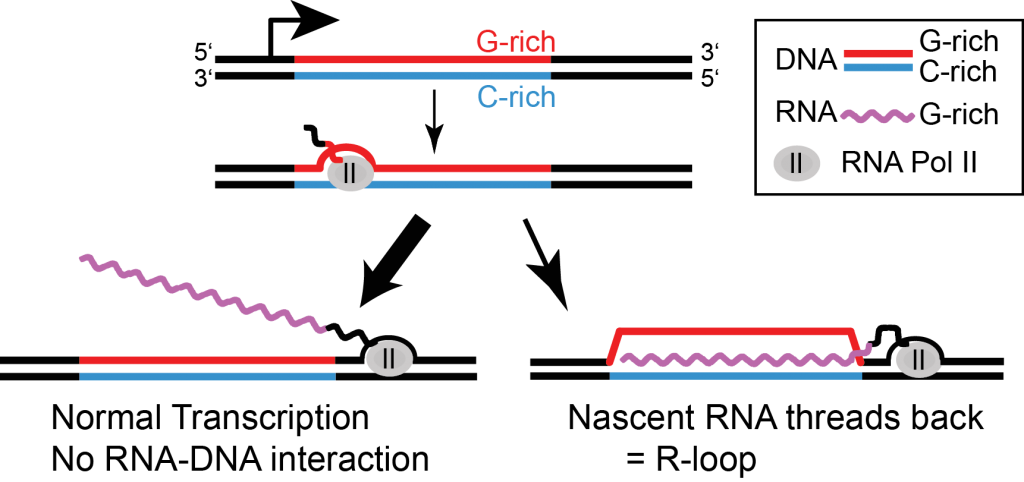
\includegraphics[width=10cm]{images/r-loops/Entanglement-1024x482.png}
	\centering
	\caption{}
	\label{fig:1}
\end{figure}


\section{Insert design}

The overall goal of this series of experiments is to transcribe carefully controlled DNA sequences, referred to as inserts, in order to systematically observe the effects of these sequences on R-loop formation \emph{in vitro}. Inserts are composed of two types of DNA components, the variable region and flanking infrastructure regions. The variable region contains the sequence we are interested in observing R-loop dynamics over. Infrastructure sequences are additional nucleotide blocks that allow for the insertion of variable regions into specific plasmid backbones in a modular fashion. 

\begin{figure}[H]
	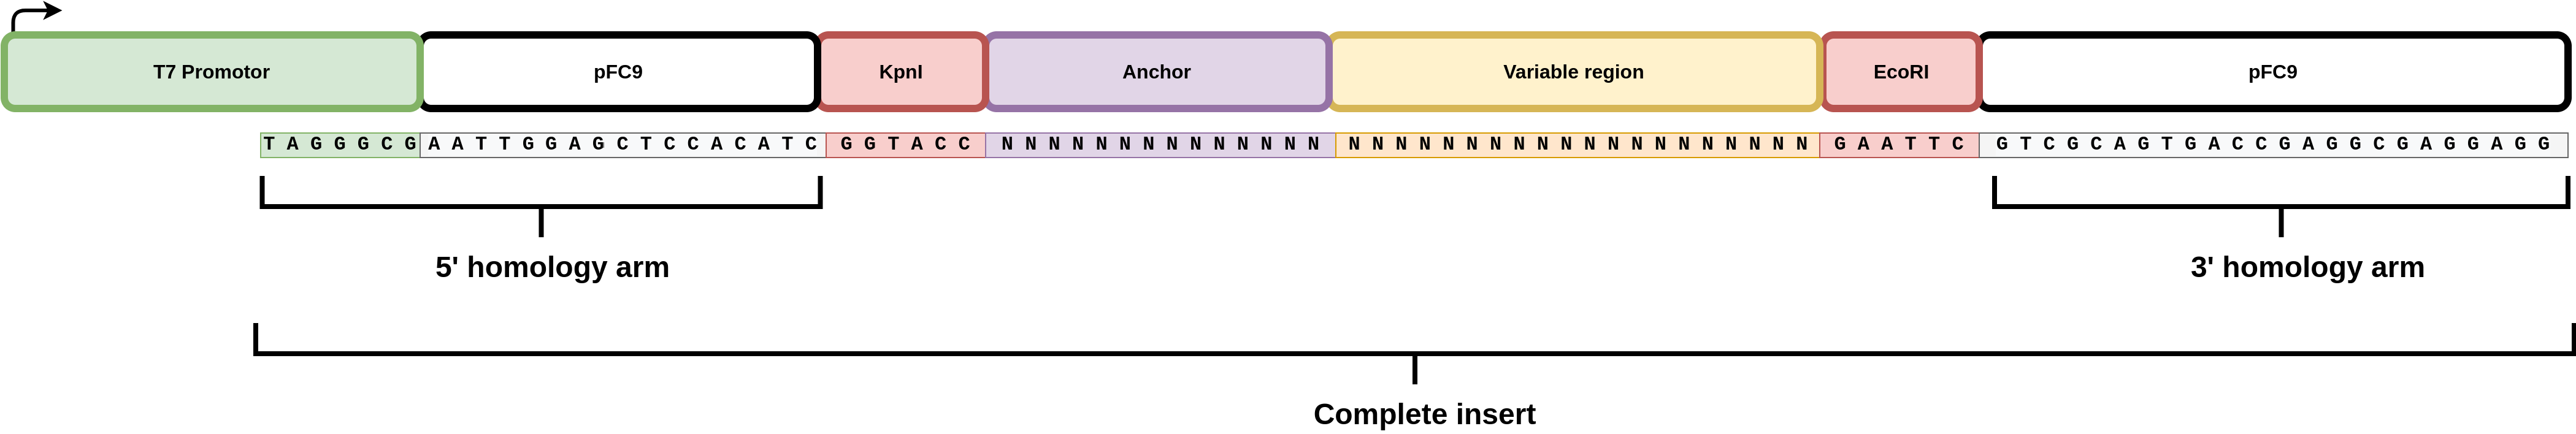
\includegraphics[width=16cm]{images/variable_region/construct_diagrams-Detailed-Insert.png}
	\centering
	\caption{Diagram of a complete insert. Colored boxes represent features insert sequences are derived from while colored sequences represent the actual nucleotide sequence.}
	\label{fig:1}
\end{figure}

From right to left (5' to 3') each insert will contain a 5' homology arm with complementary to the last 7 nucleotides of the T7 promoter, 17 nucleotides complementary to the pFC9 plasmid immediately downstream of the T7 promoter for a total of 24 bp. This will be followed by a KpnI recognition site, and an "anchor" region will will be composed of a constant sequence which can be utilized for targeting by PCR primers. The following region will contain the variable region which defines the identity of each complete insert. Finally a EcoRI recognition site and 24 taken from the region downstream of pFC9's EcoRI recognition site will be included. This design will allow for insertion of variable regions in either forward or reverse orientations using combinations of Gibson and restriction enzyme cloning, as well as allowing for later extraction via PCR or restriction enzymes. Specific methodolgies are discussed in greater detail in section \ref{}. Each insert will be completely synthesized as double strand DNA from an outside company and therefore require no additional assembly. 

\subsection{Insert components}

\subsubsection{5' homology arm and KpnI recognition site}

The first 30 bp of each insert will be composed of the 5' homology arm and a KpnI recognition site. These sequences are included to facilitate Gibson and restriction enzyme cloning into pFC9 and pFC9 respectively. These 30 bp are taken directly from nucleotides 27 - 56 of pFC9.

\begin{figure}[h]
	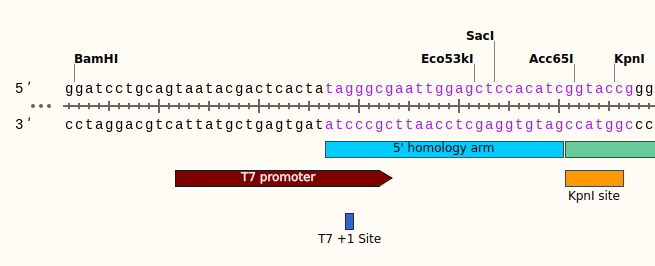
\includegraphics[width=12cm]{images/variable_region/5_homology_arm.png}
	\centering
	\caption{Location in pFC9 from which the 5' homology arm and KpnI site are modeled after. The entire 30 bp sequence is shown in purple with the 5' homology arm highlighted as a feature in blue and the KnpI site in orange.}
	\label{fig:1}
\end{figure}


\subsection{Anchor}

The anchor region serves as a constant sequence that will always be present in any final assembled construct adjacent to the 5' end of the variable region. Having this region within the insertion sequence means for a given plasmid backbone, at most, 1 pair of primers will be required to amplify any sequence downstream of the 3' end of the anchor. This is useful when working with libraries containing all insertion sequences as each unique insertion will not require its own primer pair to amplify. This utility is more explicitly shown in sections \ref{} and \ref{}. 

Since this region is intended to be used as part of a PCR primer done to make sure it was unique across all plasmid backbones and insert sequences and did not contain any restriction enzyme recognition sites used in any of the cloning experiments. 

\subsection{Variable regions}

Each insert will contain 1 variable region which will be designed to test the effects of different sequence properties on R-loop dynamics, namely GC / AT skew, GC content and G / C clustering. Each variable region will be 200 bp in length. Twenty nine different variable regions with the properties described in table \ref{table:1} will be generated using the \href{https://github.com/EthanHolleman/plasmid-VR-design}{variable region design workflow}. Each variable region, as part of the larger insertion sequence, will be cloned downstream of a promoter so it is transcribed in the forward direction. 

\begin{table}
\centering
\caption{Properties of all syntheized inserts. The G clustering number refers to the number of G nucleotides in a given cluster with 0 being no clustering.}
\label{table:1}
\begin{tabular}{rrrrrr}
\toprule=
 GC Skew &  AT Skew &  GC Content &  G Clustering &  Reverse Complement &  Insert Number \\
\midrule
     0.2 &      0.0 &         0.4 &             0 &                   1 &              0 \\
     0.1 &      0.0 &         0.3 &             0 &                   0 &              1 \\
     0.6 &      0.0 &         0.6 &             0 &                   0 &              2 \\
     0.4 &      0.0 &         0.3 &             0 &                   1 &              3 \\
     0.2 &      0.0 &         0.3 &             0 &                   1 &              4 \\
     0.0 &      0.0 &         0.3 &             0 &                   1 &              5 \\
     0.0 &      0.0 &         0.6 &             0 &                   0 &              6 \\
     0.6 &      0.0 &         0.5 &             0 &                   0 &              7 \\
     0.1 &      0.0 &         0.6 &             0 &                   0 &              8 \\
     0.4 &      0.0 &         0.6 &             0 &                   0 &              9 \\
     0.2 &      0.0 &         0.6 &             0 &                   0 &             10 \\
     0.0 &      0.0 &         0.5 &             0 &                   1 &             11 \\
     0.6 &      0.0 &         0.4 &             0 &                   0 &             12 \\
     0.0 &      0.0 &         0.4 &             0 &                   1 &             13 \\
     0.1 &      0.0 &         0.5 &             0 &                   0 &             14 \\
     0.6 &      0.0 &         0.3 &             0 &                   0 &             15 \\
     0.4 &      0.0 &         0.5 &             0 &                   1 &             16 \\
     0.2 &      0.0 &         0.5 &             0 &                   1 &             17 \\
     0.1 &      0.0 &         0.4 &             0 &                   0 &             18 \\
     0.4 &      0.0 &         0.4 &             0 &                   1 &             19 \\
     0.4 &      0.0 &         0.6 &             2 &                   1 &             20 \\
     0.4 &      0.2 &         0.6 &             2 &                   1 &             21 \\
     0.4 &      0.4 &         0.6 &             2 &                   1 &             22 \\
     0.4 &      0.0 &         0.6 &             3 &                   1 &             23 \\
     0.4 &      0.2 &         0.6 &             3 &                   1 &             24 \\
     0.4 &      0.4 &         0.6 &             3 &                   1 &             25 \\
     0.4 &      0.0 &         0.6 &             4 &                   1 &             26 \\
     0.4 &      0.2 &         0.6 &             4 &                   1 &             27 \\
     0.4 &      0.4 &         0.6 &             4 &                   1 &             28 \\
\bottomrule
\end{tabular}
\end{table}


A subset of the variable regions will also be cloned further downstream of the same promoter species and oriented so the reverse complement of the sequence is transcribed in order to access these regions capacity for R-loop termination. The properties of the transcripts of these sequences are listed in table \ref{table:2}. 

\begin{table}[H]
\centering
\caption{}
\label{table:2}
\begin{tabular}{rrrrr}
\toprule
 GC Skew &  AT Skew &  GC Content &  C Clustering &  Reverse Complement of Insert \\
\midrule
    -0.2 &     -0.0 &         0.4 &             0 &                             0 \\
    -0.4 &     -0.0 &         0.3 &             0 &                             3 \\
    -0.2 &     -0.0 &         0.3 &             0 &                             4 \\
    -0.0 &     -0.0 &         0.3 &             0 &                             5 \\
    -0.0 &     -0.0 &         0.5 &             0 &                            11 \\
    -0.0 &     -0.0 &         0.4 &             0 &                            13 \\
    -0.4 &     -0.0 &         0.5 &             0 &                            16 \\
    -0.2 &     -0.0 &         0.5 &             0 &                            17 \\
    -0.4 &     -0.0 &         0.4 &             0 &                            19 \\
    -0.4 &     -0.0 &         0.6 &             2 &                            20 \\
    -0.4 &     -0.2 &         0.6 &             2 &                            21 \\
    -0.4 &     -0.4 &         0.6 &             2 &                            22 \\
    -0.4 &     -0.0 &         0.6 &             3 &                            23 \\
    -0.4 &     -0.2 &         0.6 &             3 &                            24 \\
    -0.4 &     -0.4 &         0.6 &             3 &                            25 \\
    -0.4 &     -0.0 &         0.6 &             4 &                            26 \\
    -0.4 &     -0.2 &         0.6 &             4 &                            27 \\
    -0.4 &     -0.4 &         0.6 &             4 &                            28 \\
\bottomrule
\end{tabular}
\end{table}


The cloning experiments required to produce these termination constructs will be undertaken after initiation experiments are completed. This will allow for the identification of a strong initiation sequence that can be used to reliablely initiated R-loops in order to study their downstream termination. 

\begin{table}
\centering
\caption{}
\label{table:3}
\begin{tabular}{rr}
\toprule
 Total synthesized inserts &  Total contructs \\
\midrule
                        29 &               47 \\
\bottomrule
\end{tabular}
\end{table}


While the global sequence properties for each variable region are well defined, properties such as GC-skew, content or clustering do not determine what nucleotide should occur at position \emph{n} in a given sequence. In this way, the parameters that define and separate each variable region can be thought of as bounding the set of all possible nucleotide sequences of length 200. In order one specific sequence from this set we can sample a large number of sequences and access each one with metrics relevant to the realities of the cloning protocols and R-loop formation. 


\subsubsection{Restriction enzyme recognition sites}

Over the course of all planned cloning experiments, all the restriction enzymes in table \ref{} will be utilized in some capacity. It is therefore critical that the inserts are not cut unexpectedly within the variable region by any of these enzymes. Accordingly, before passing on for further downstream analysis potential variable regions containing any of these recognition sites were thrown out. 

\begin{table}[H]
	\caption{}
	\centering
	\begin{tabular}{@{}ll@{}}
		\toprule
		Enzyme  & Recognition sequence \\ \midrule
		KnpI    & GGTACC               \\
		EcoRI   & GAATTC               \\
		HindIII & AAGCTT               \\ \bottomrule
	\end{tabular}
\end{table}


\subsubsection{Predicted R-loop probability}

The Chedin lab has previously devloped and the work of Dr. Robert has devloped R-looper here we are using it to access where in distrabution sequences tend to fall using predictions for average probility of R-loop formation across the length of a sequence and the mean local average energy. 

\begin{figure}[H]
	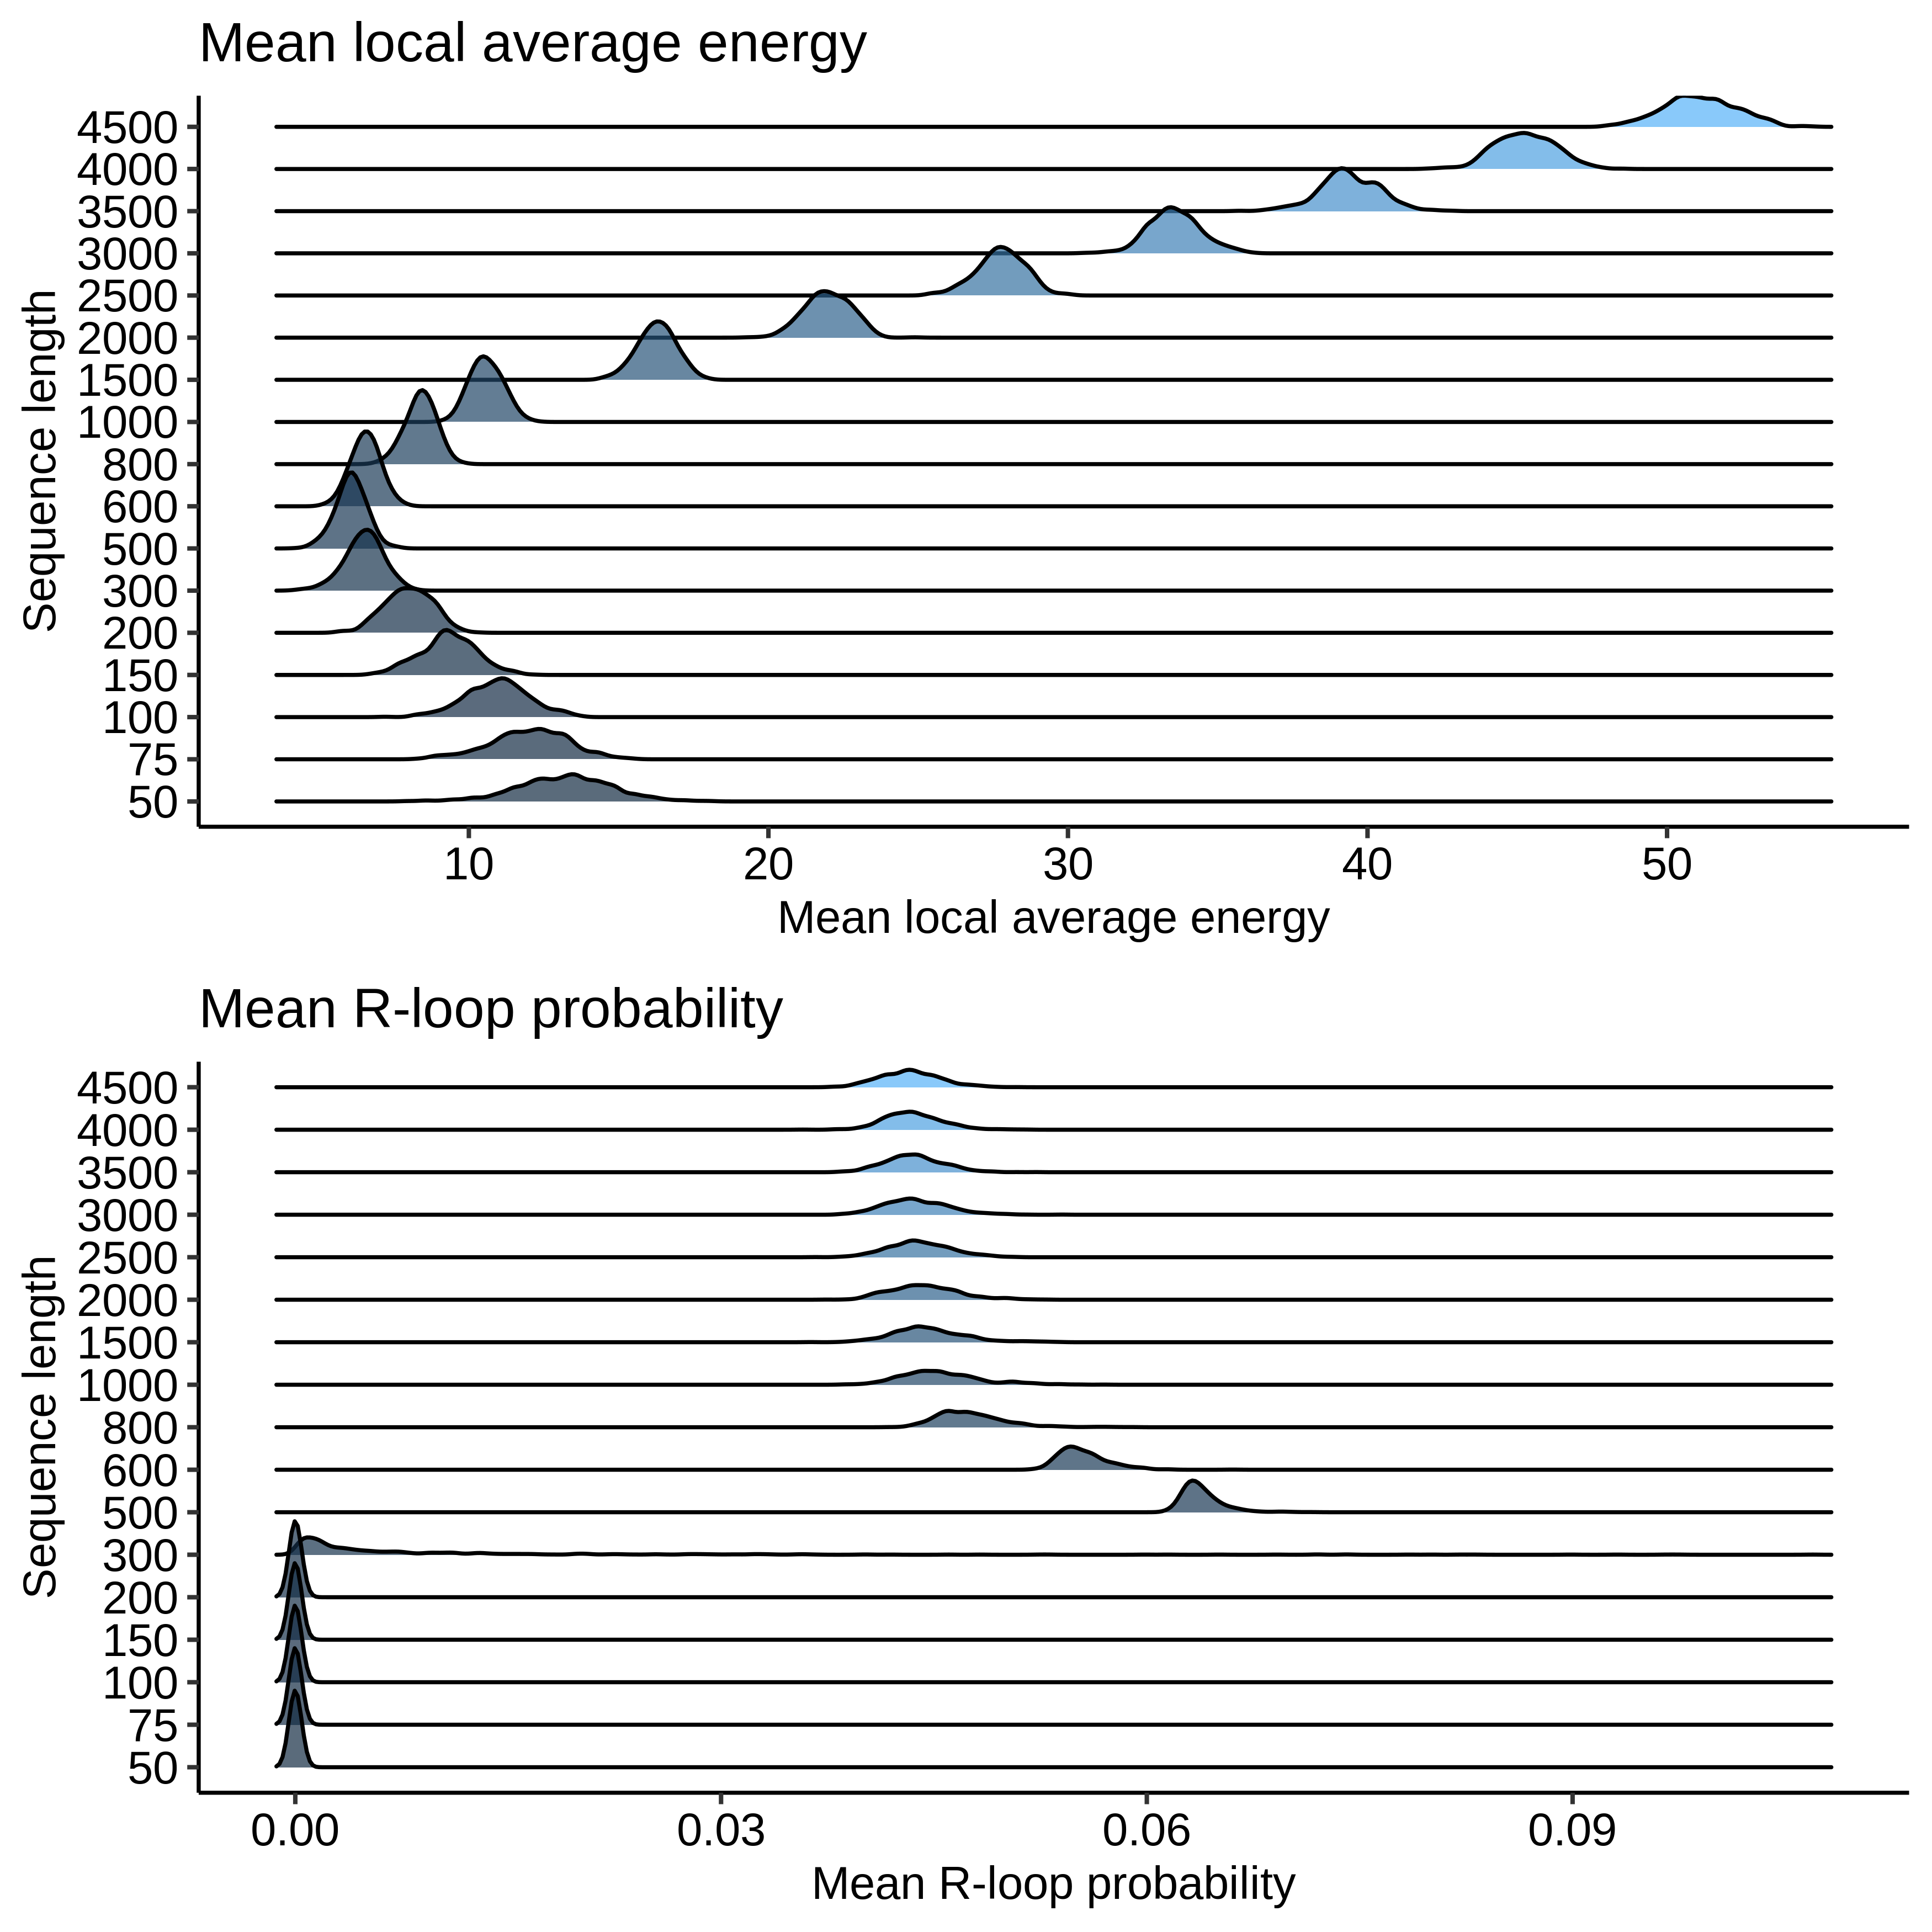
\includegraphics[width=10cm]{images/plots/rand_seq_LAE_dist.png}
	\centering
	\caption{Map of pFC9 showing major features and all restriction enzyme recognition sites.}
	\label{fig:pFC9}
\end{figure}

\subsubsection{RNA secondary structure}

Significant amounts of RNA secondary structure, especially large hairpins, can be expected to reduce the likelihood of R-loop formation by causing competition for binding to the nascent RNA strand between itself and the DNA template. 

\subsection{EcoRI site}

\subsection{3' homology arm}

\section{Assembly of DNA inserts}


\subsection{T7 initiation series constructs}
\label{T7:init} 

The first series of constructs will be utilize pFC9 as the plasmid backbone.   

\begin{figure}[H]
	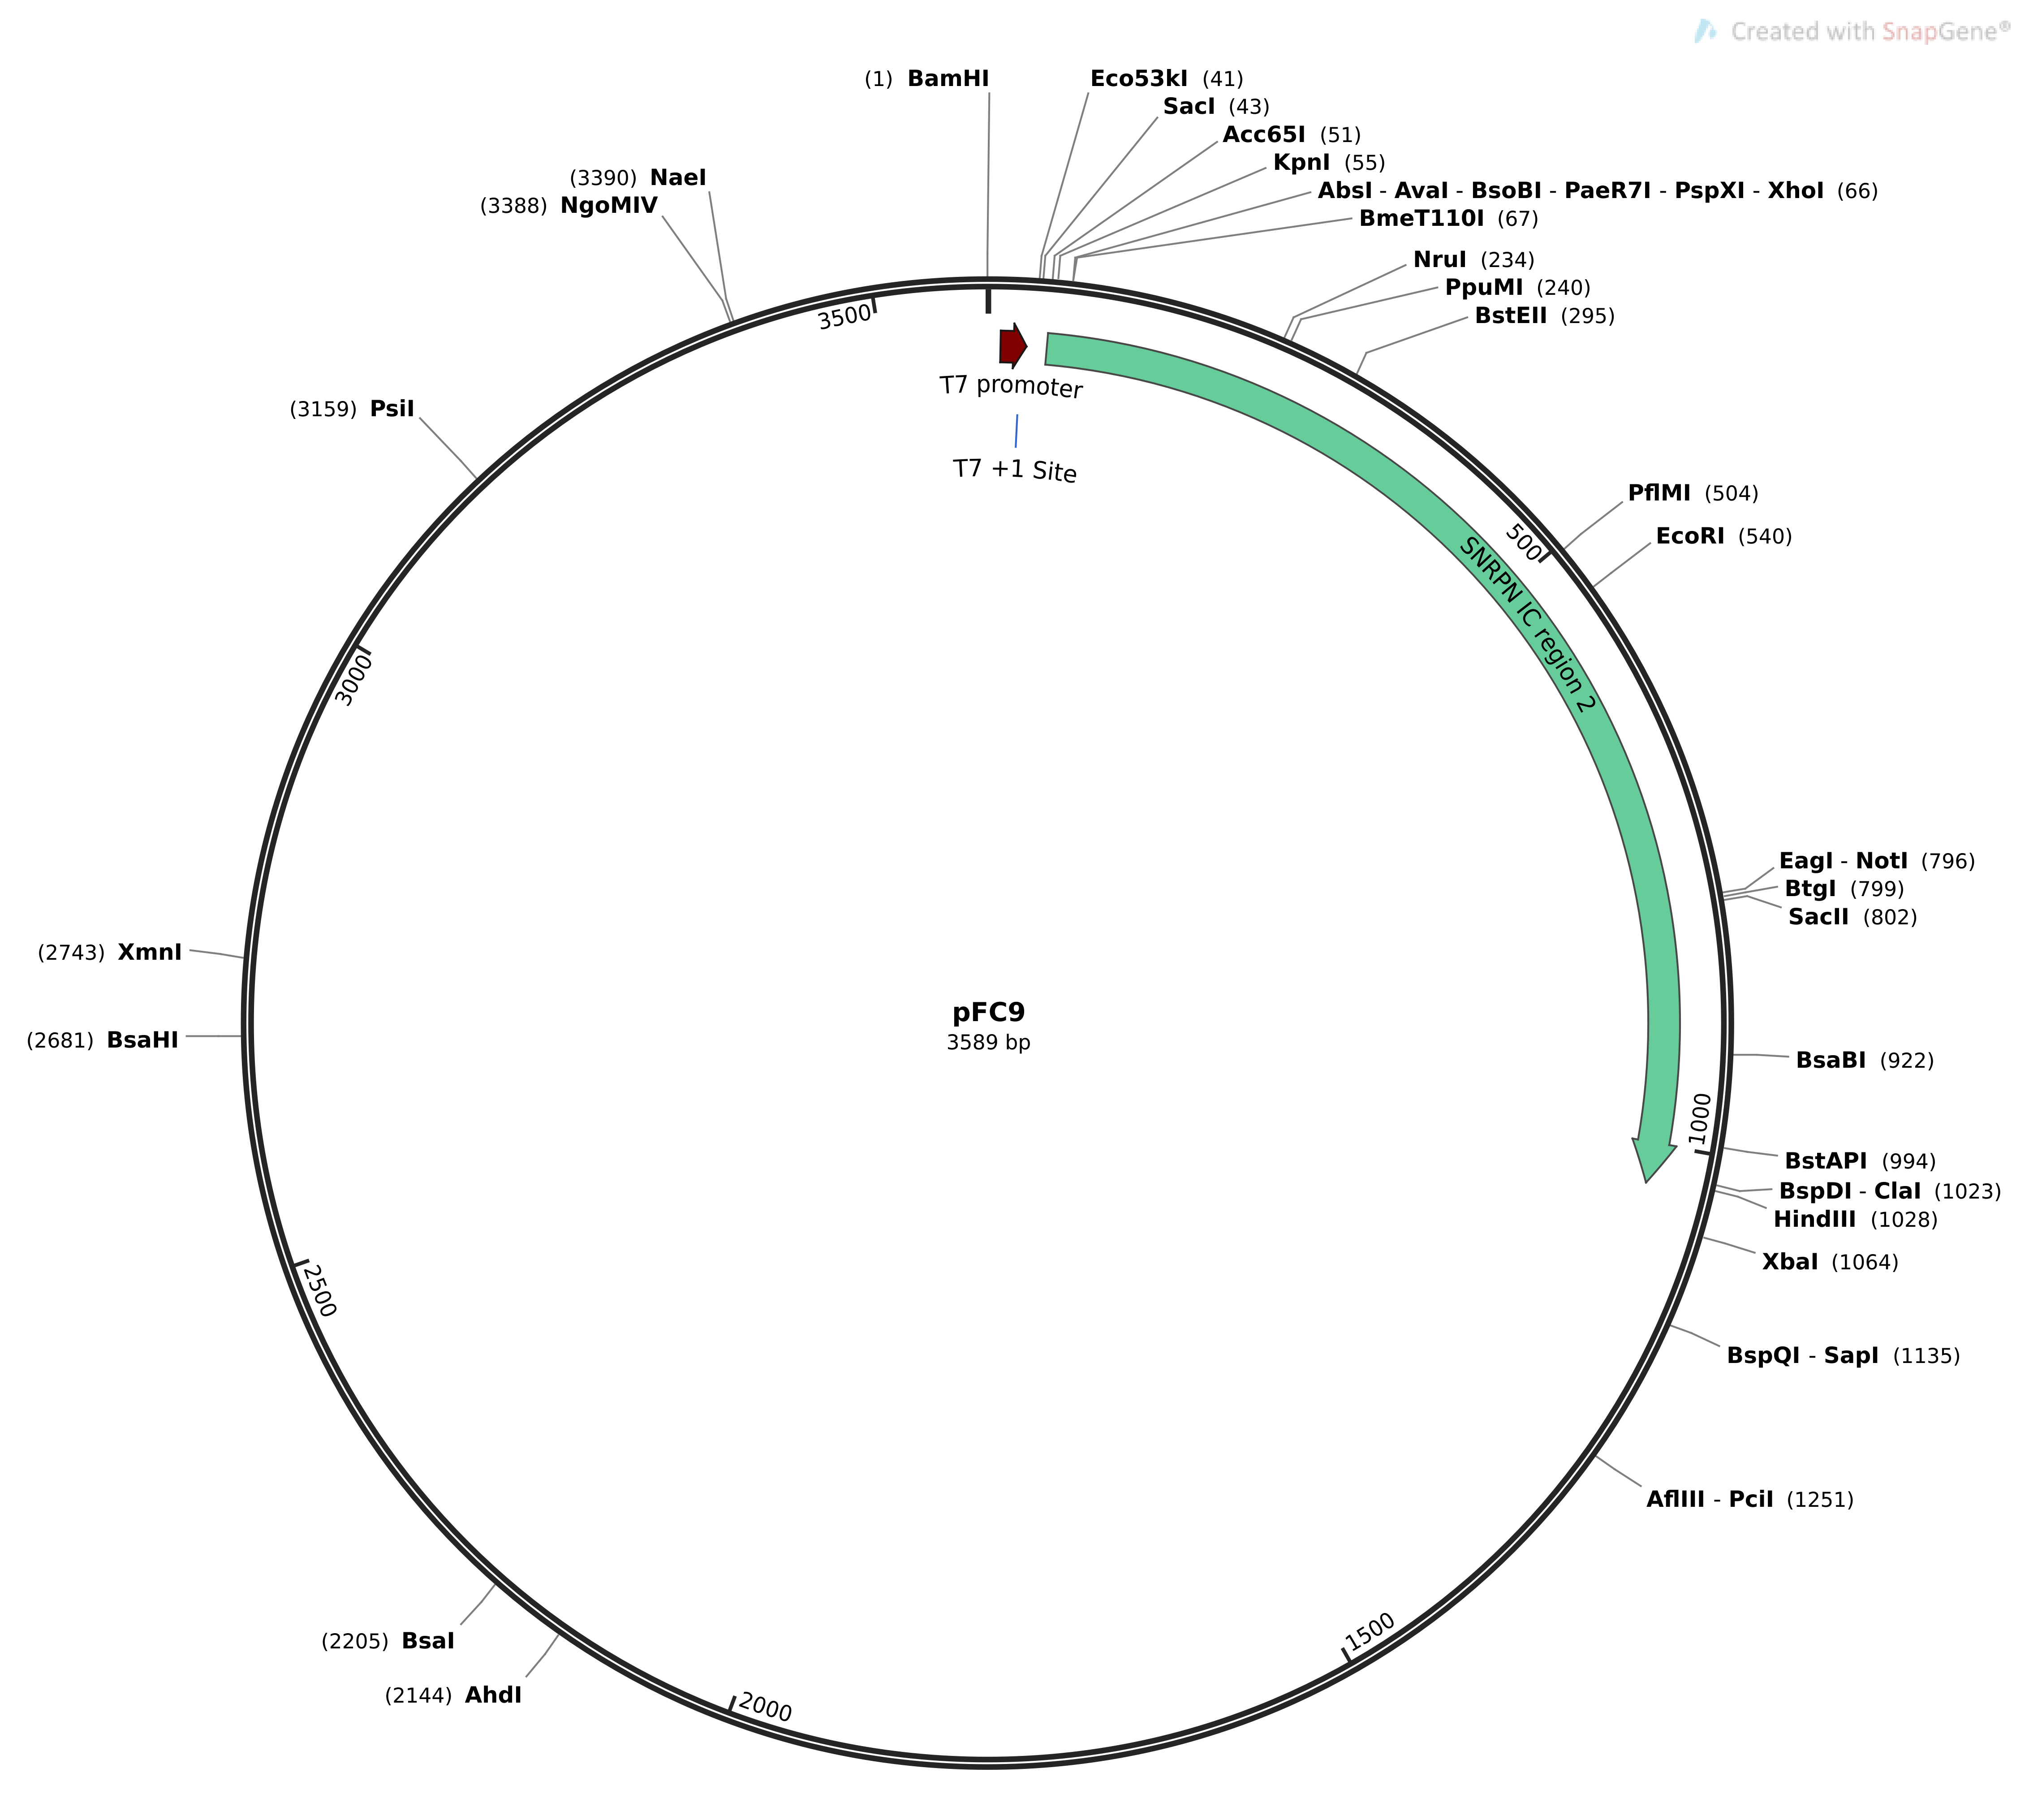
\includegraphics[width=10cm]{images/plasmid_maps/pFC9_Map.png}
	\centering
	\caption{Map of pFC9 showing major features and all restriction enzyme recognition sites.}
	\label{fig:pFC9}
\end{figure}

First, pFC9 will be cut using Eco53KI, producing blunt ends just downstream of the T7 promotor (fig \ref{fig:pFC9}). The complete ensemble of inserts will then be added in equal concentrations. Using the \href{https://www.neb.com/protocols/2012/12/11/gibson-assembly-protocol-e5510}{NEB Gibson assembly kit and protocol}, the 5' and 3' homology arms will anneal to the T7 and extension region downstream of the Eco53KI cut site of pFC9 respectively producing a library of circular pFC9 plasmids with each insertion sequence in theoretically equivalent concentrations. 

\begin{figure}[H]
	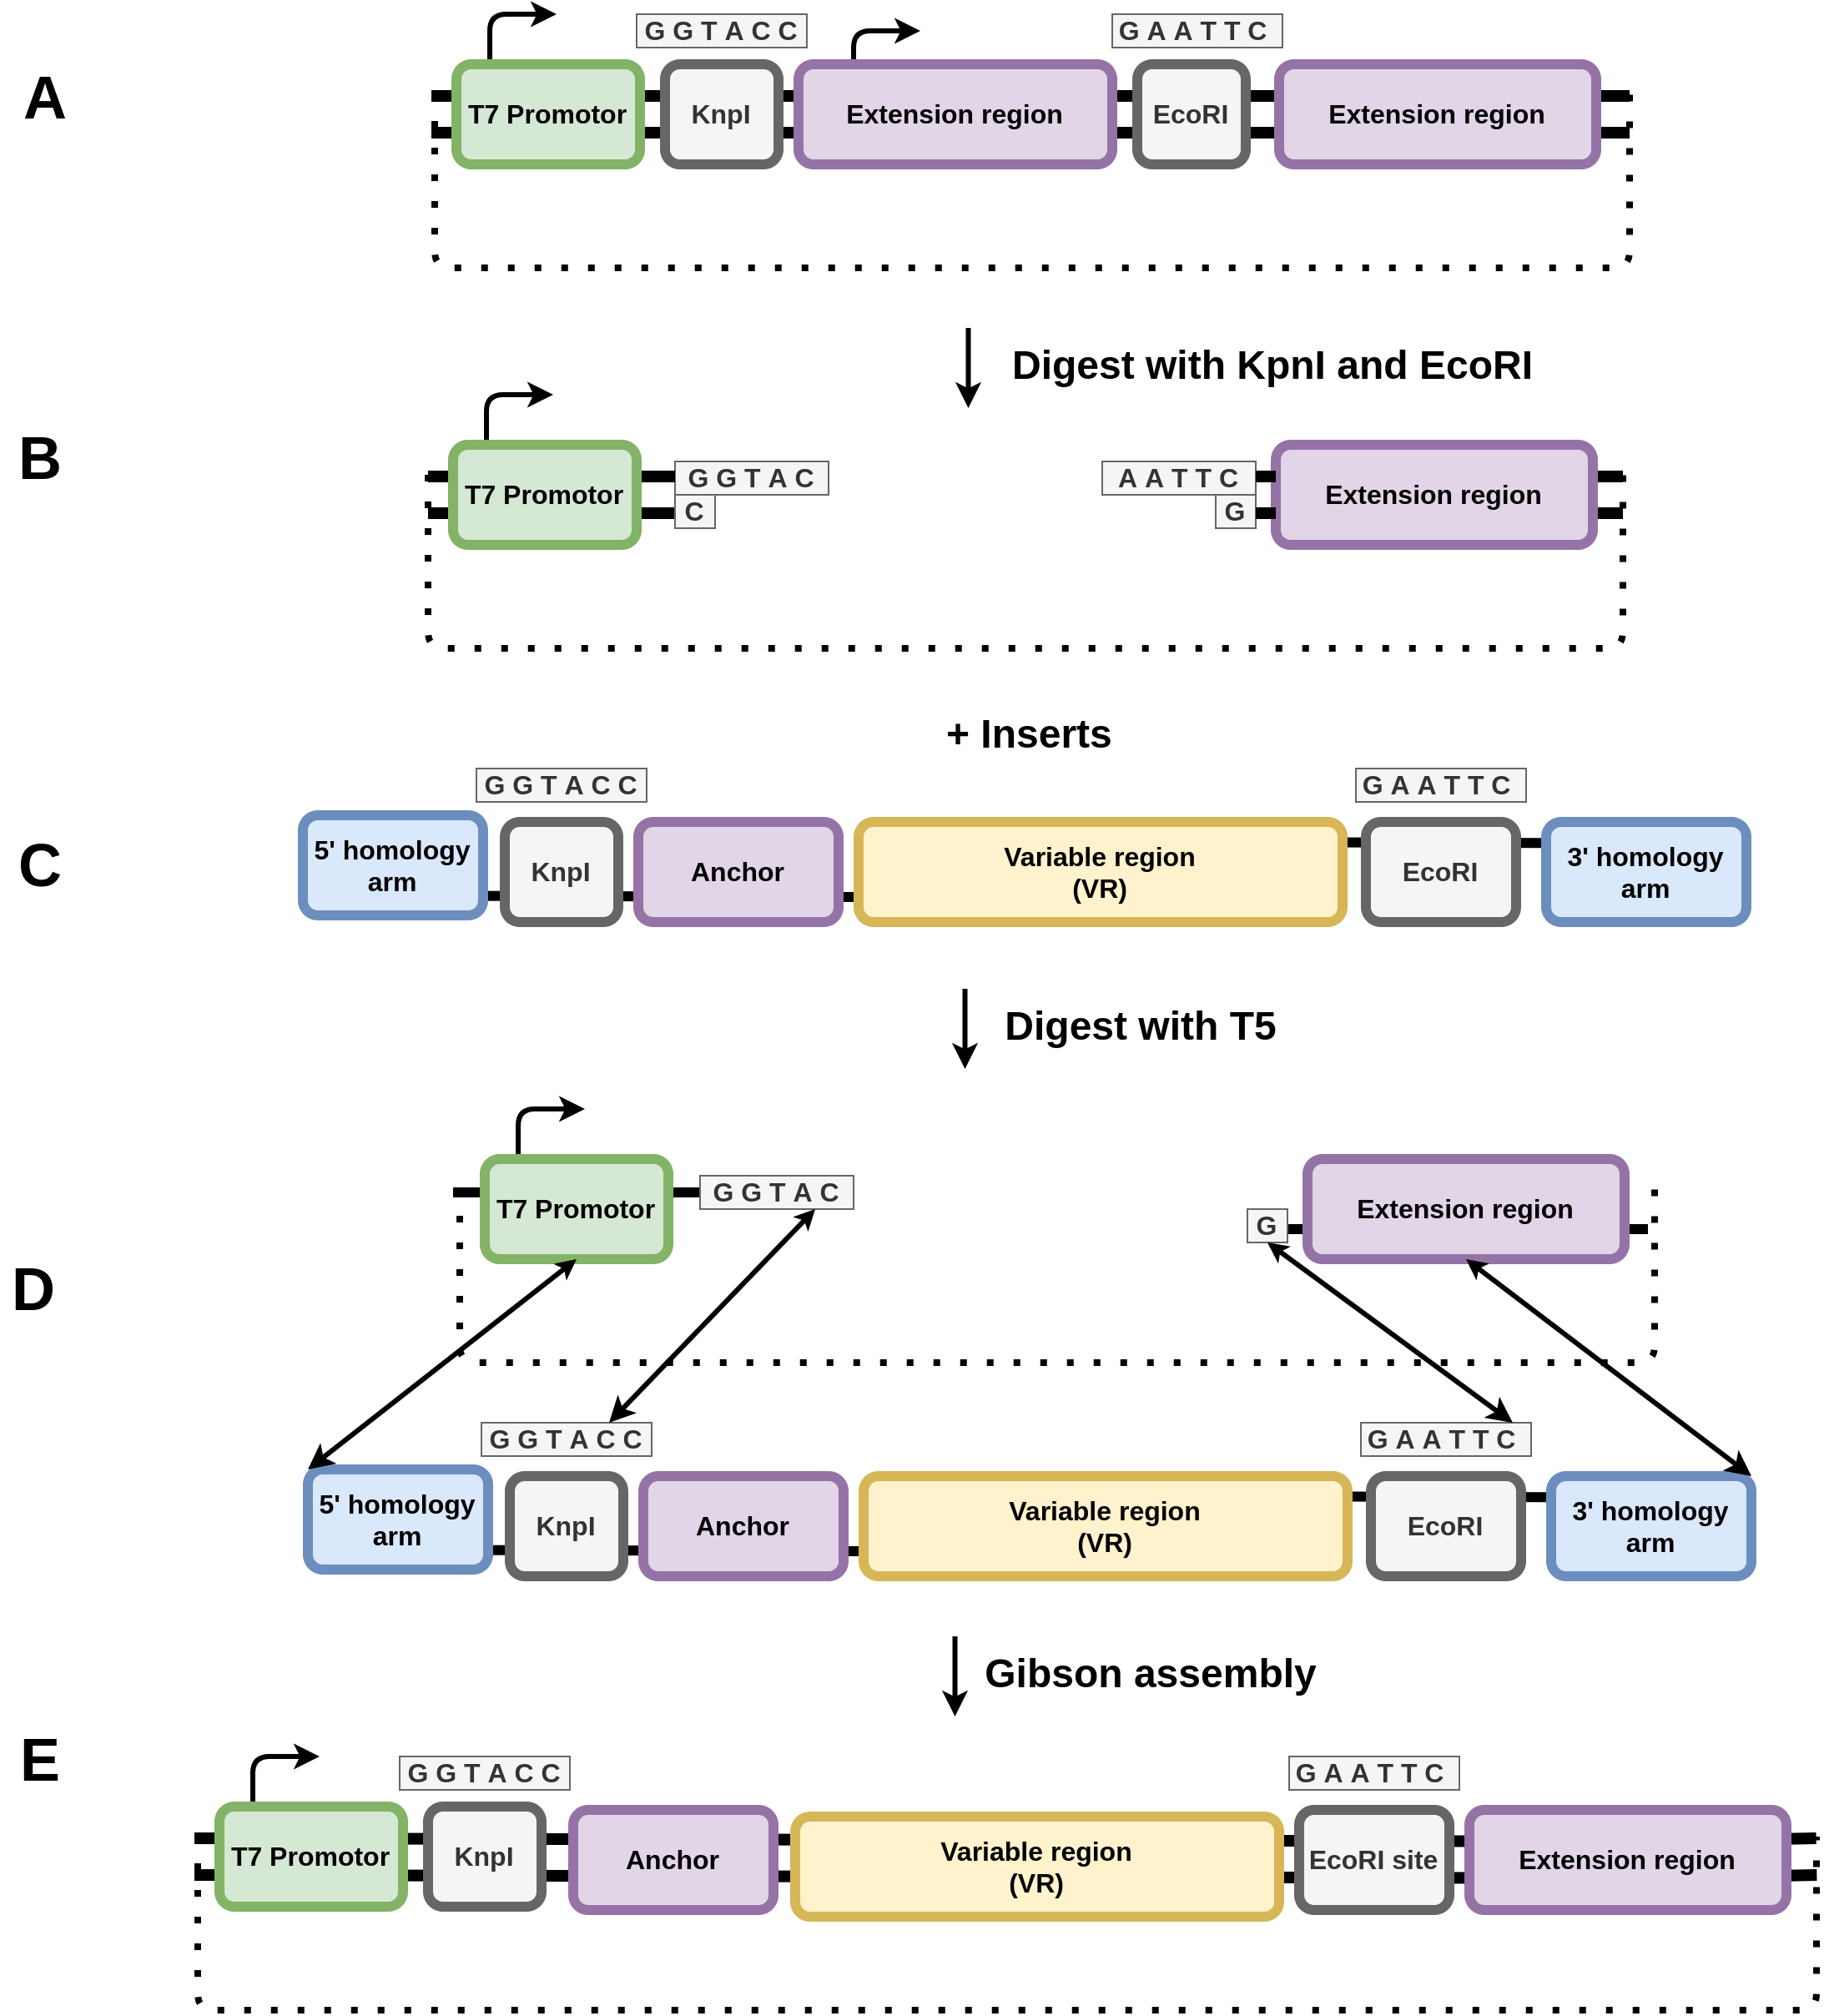
\includegraphics[width=15cm]{images/cloning_diagrams/construct_diagrams-T7-Initiation-series.png}
	\centering
	\caption{Diagram of pFC9 insertion series cloning strategy.}
\end{figure}

Primers will be designed for a subset of initiation regions and the relative concentrations of each insert will be measured by qPCR. Having confirmed that inserts are present at relatively equal concentrations the library will be transcribed \emph{in vitro} and prepared for single molecule R-loop footprinting using uniquely bar-coded PCR primers to facilitate the computational removal of PCR duplicates. 


\subsection{T7 termination series constructs}

After the successful sequencing of the T7 initiation series, pFC8 will be utilized as the backbone for construction of the termination series library. First, the strongest and most consistent R-loop initiator identified from the T7 initiation series will be cloned into pFC9 without the presence of any other inserts using the methods described in section \ref{T7:init}. 

\begin{figure}[H]
	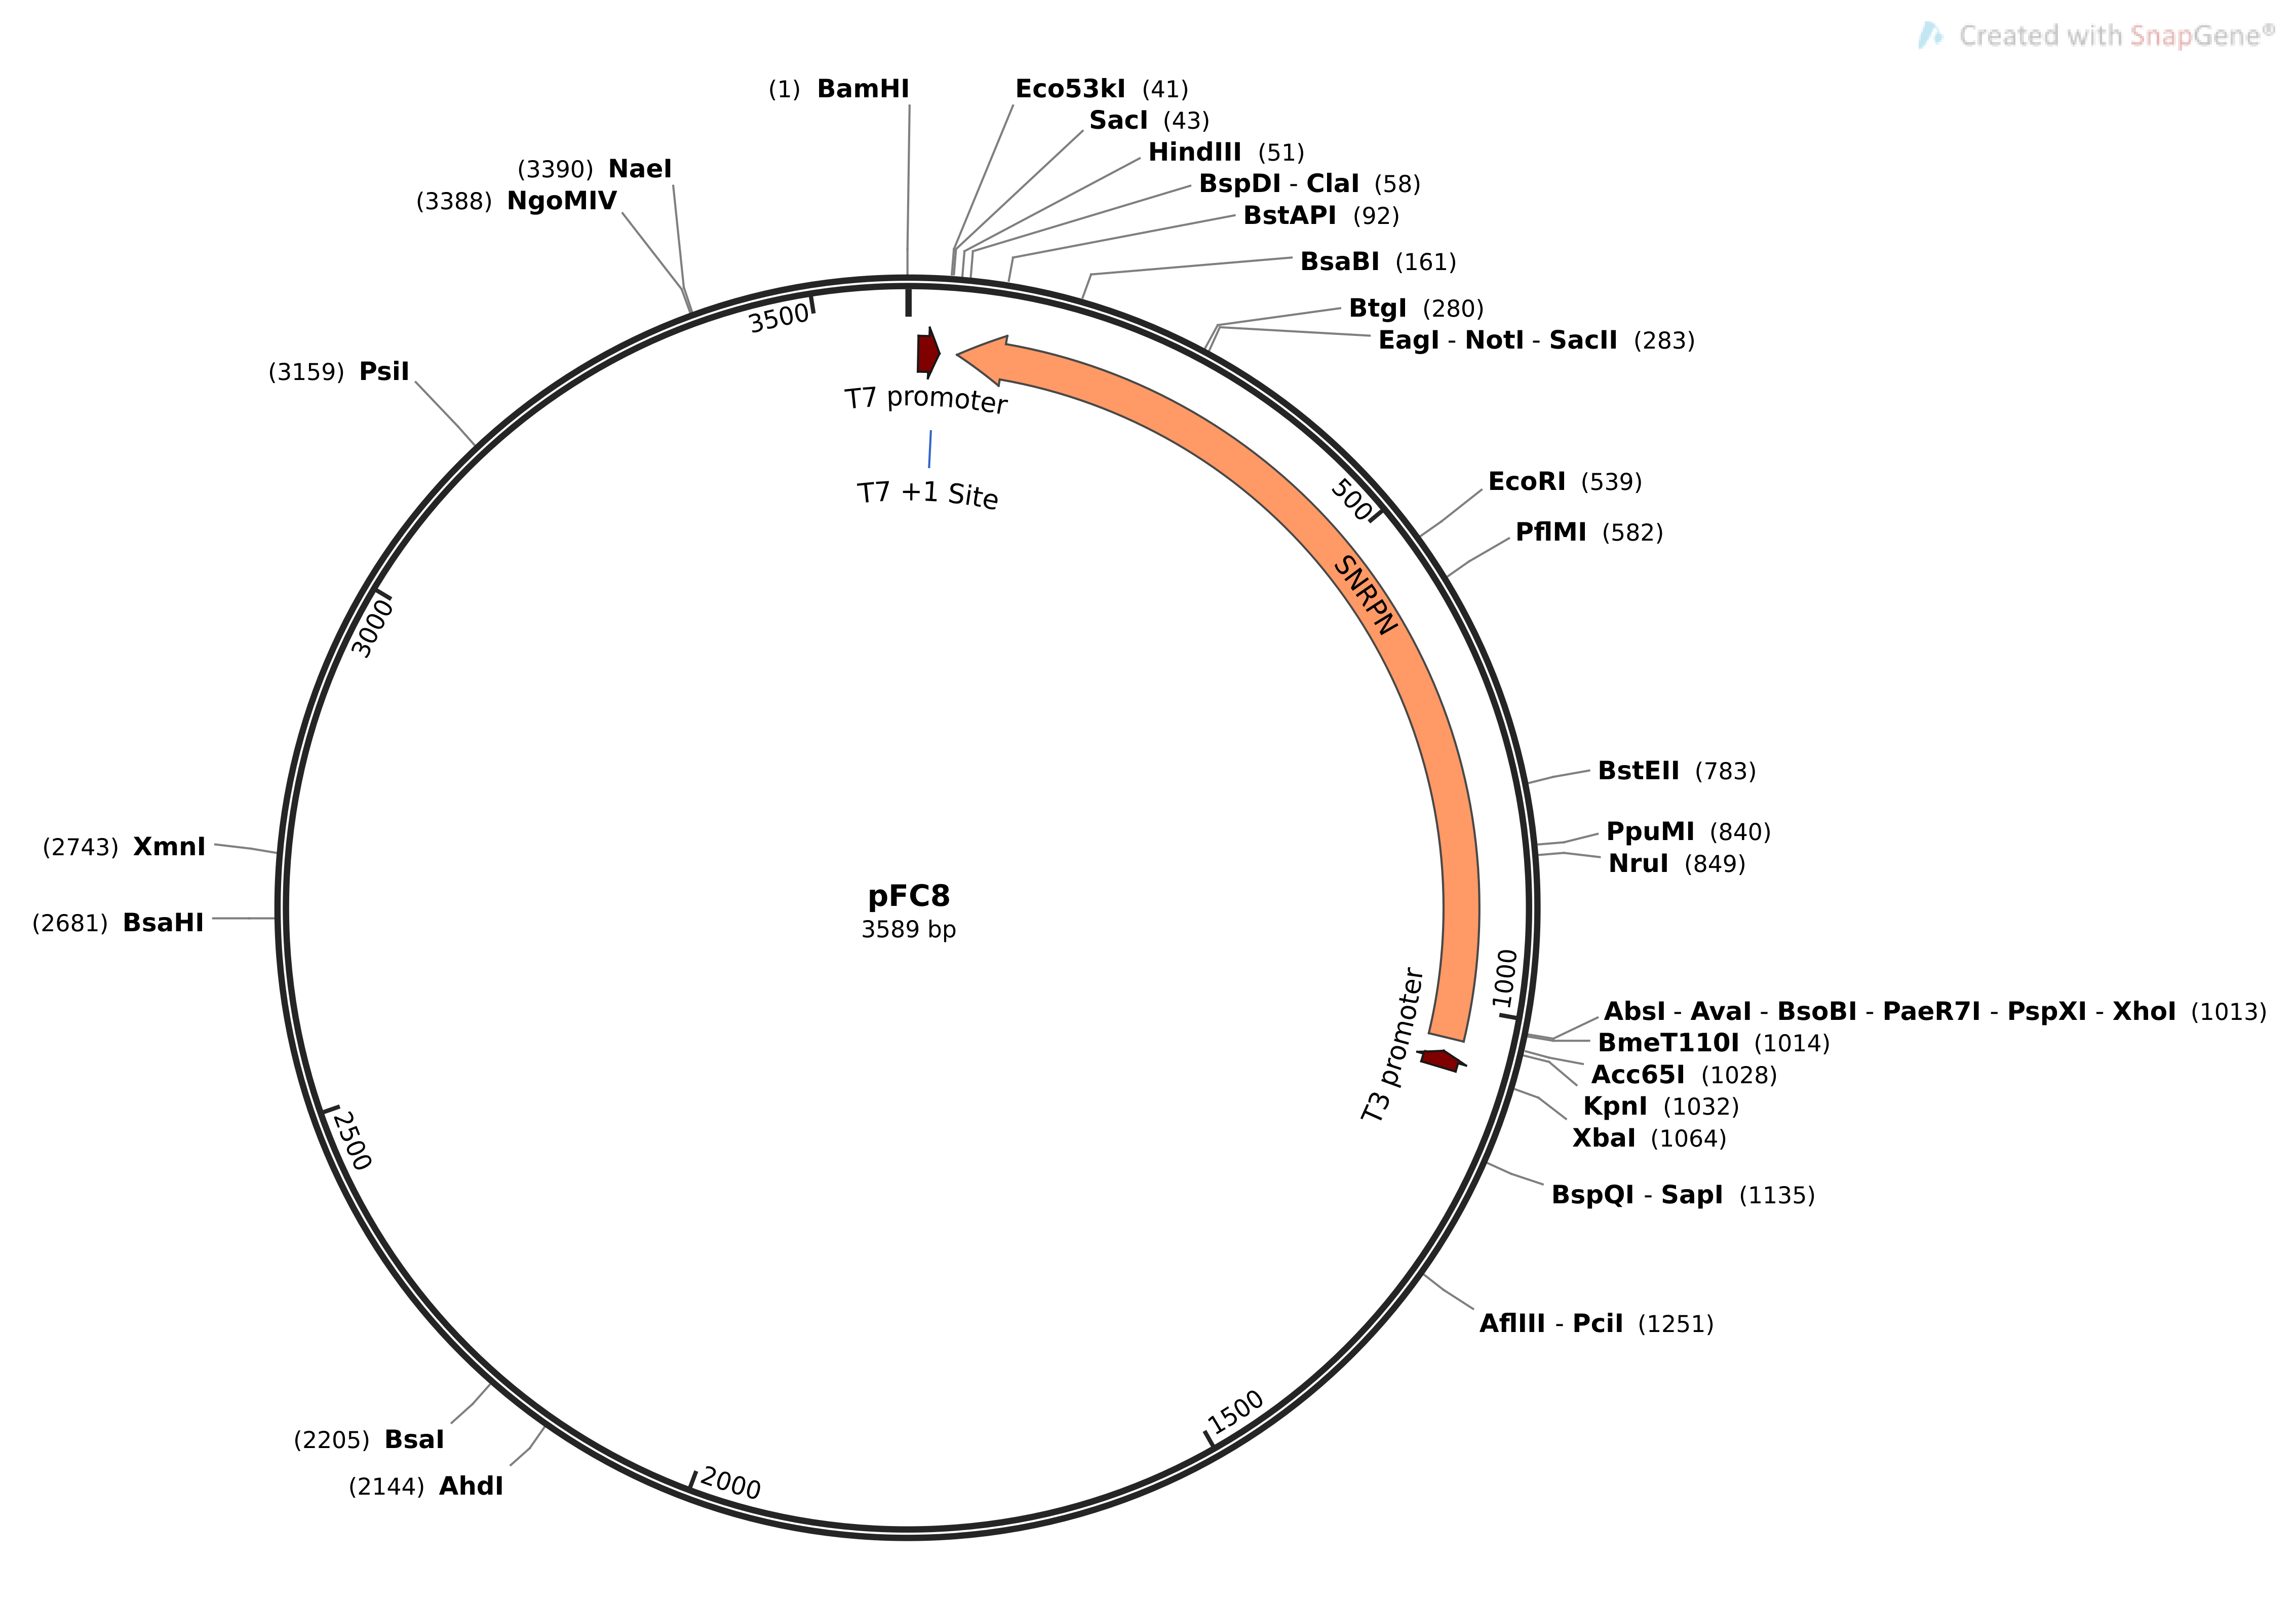
\includegraphics[width=12cm]{images/plasmid_maps/pFC8_Map.png}
	\centering
	\caption{Map of pFC8.}
	\label{fig:pFC8}
\end{figure}

\begin{figure}[H]
	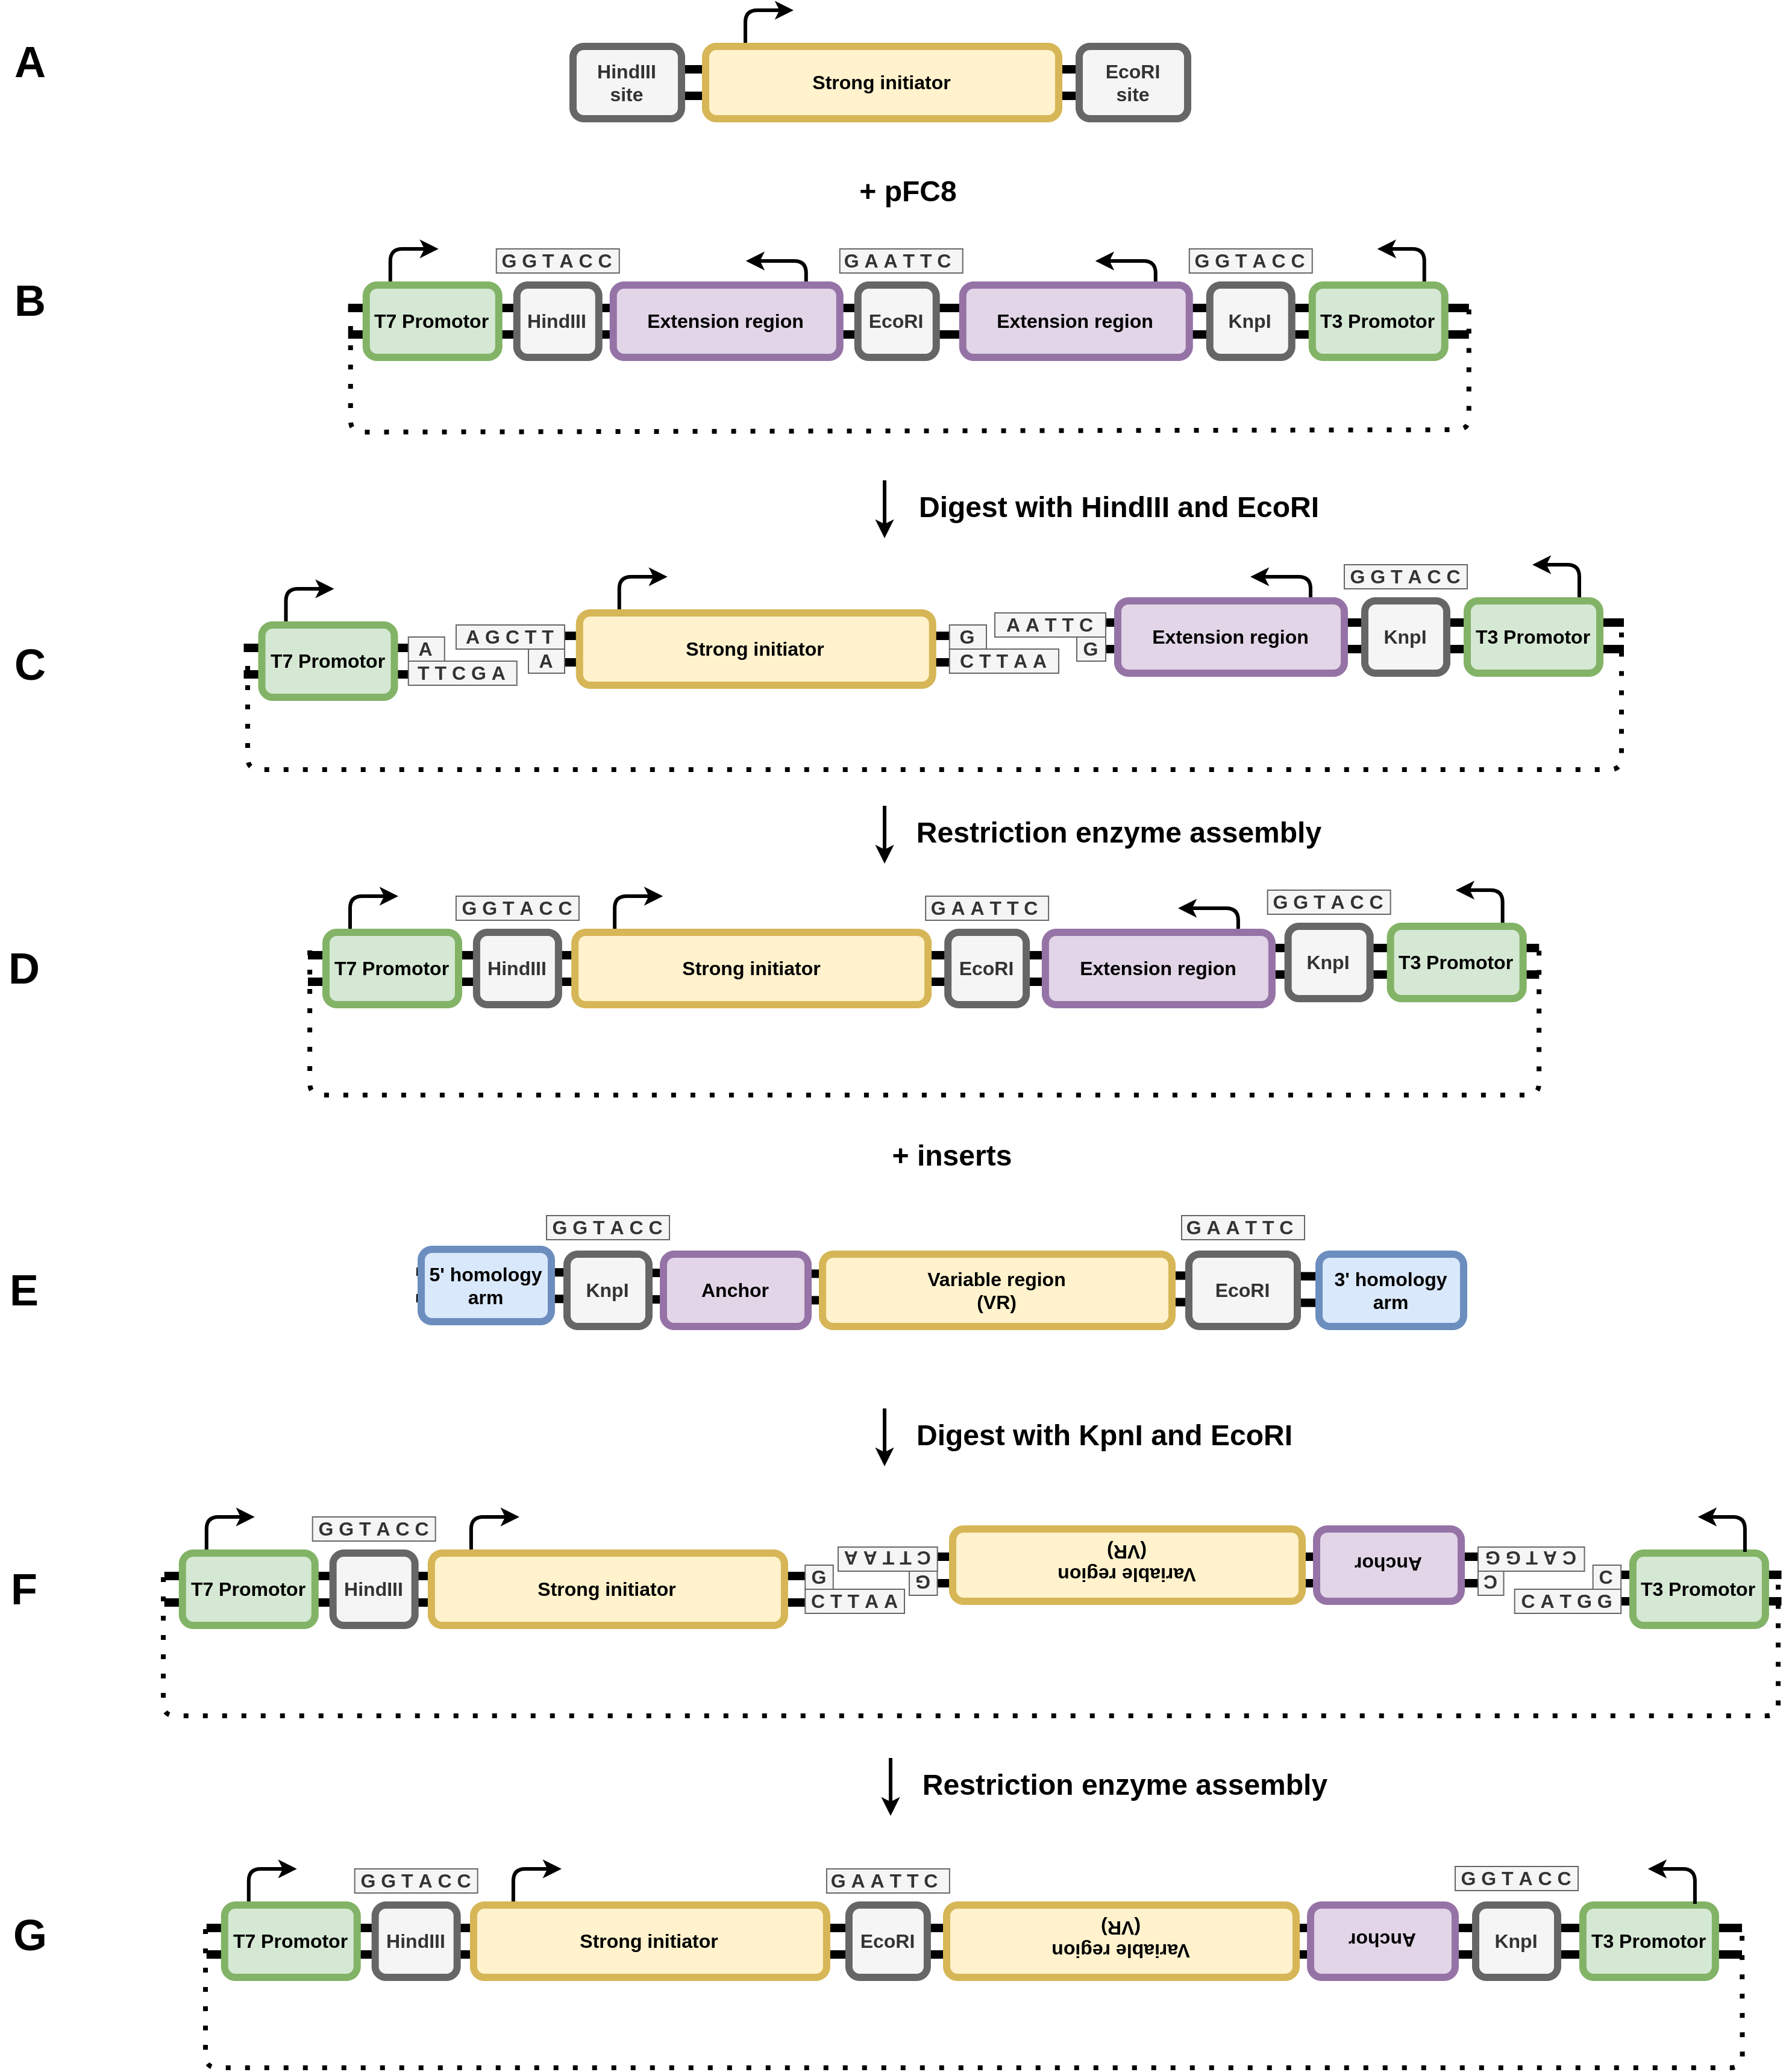
\includegraphics[width=15cm]{images/cloning_diagrams/construct_diagrams-T7-termination-series.png}
	\centering
	\caption{Diagram of pFC9 insertion series cloning strategy.}
\end{figure}


\subsection{Tac initiation series constructs}

\begin{figure}[H]
	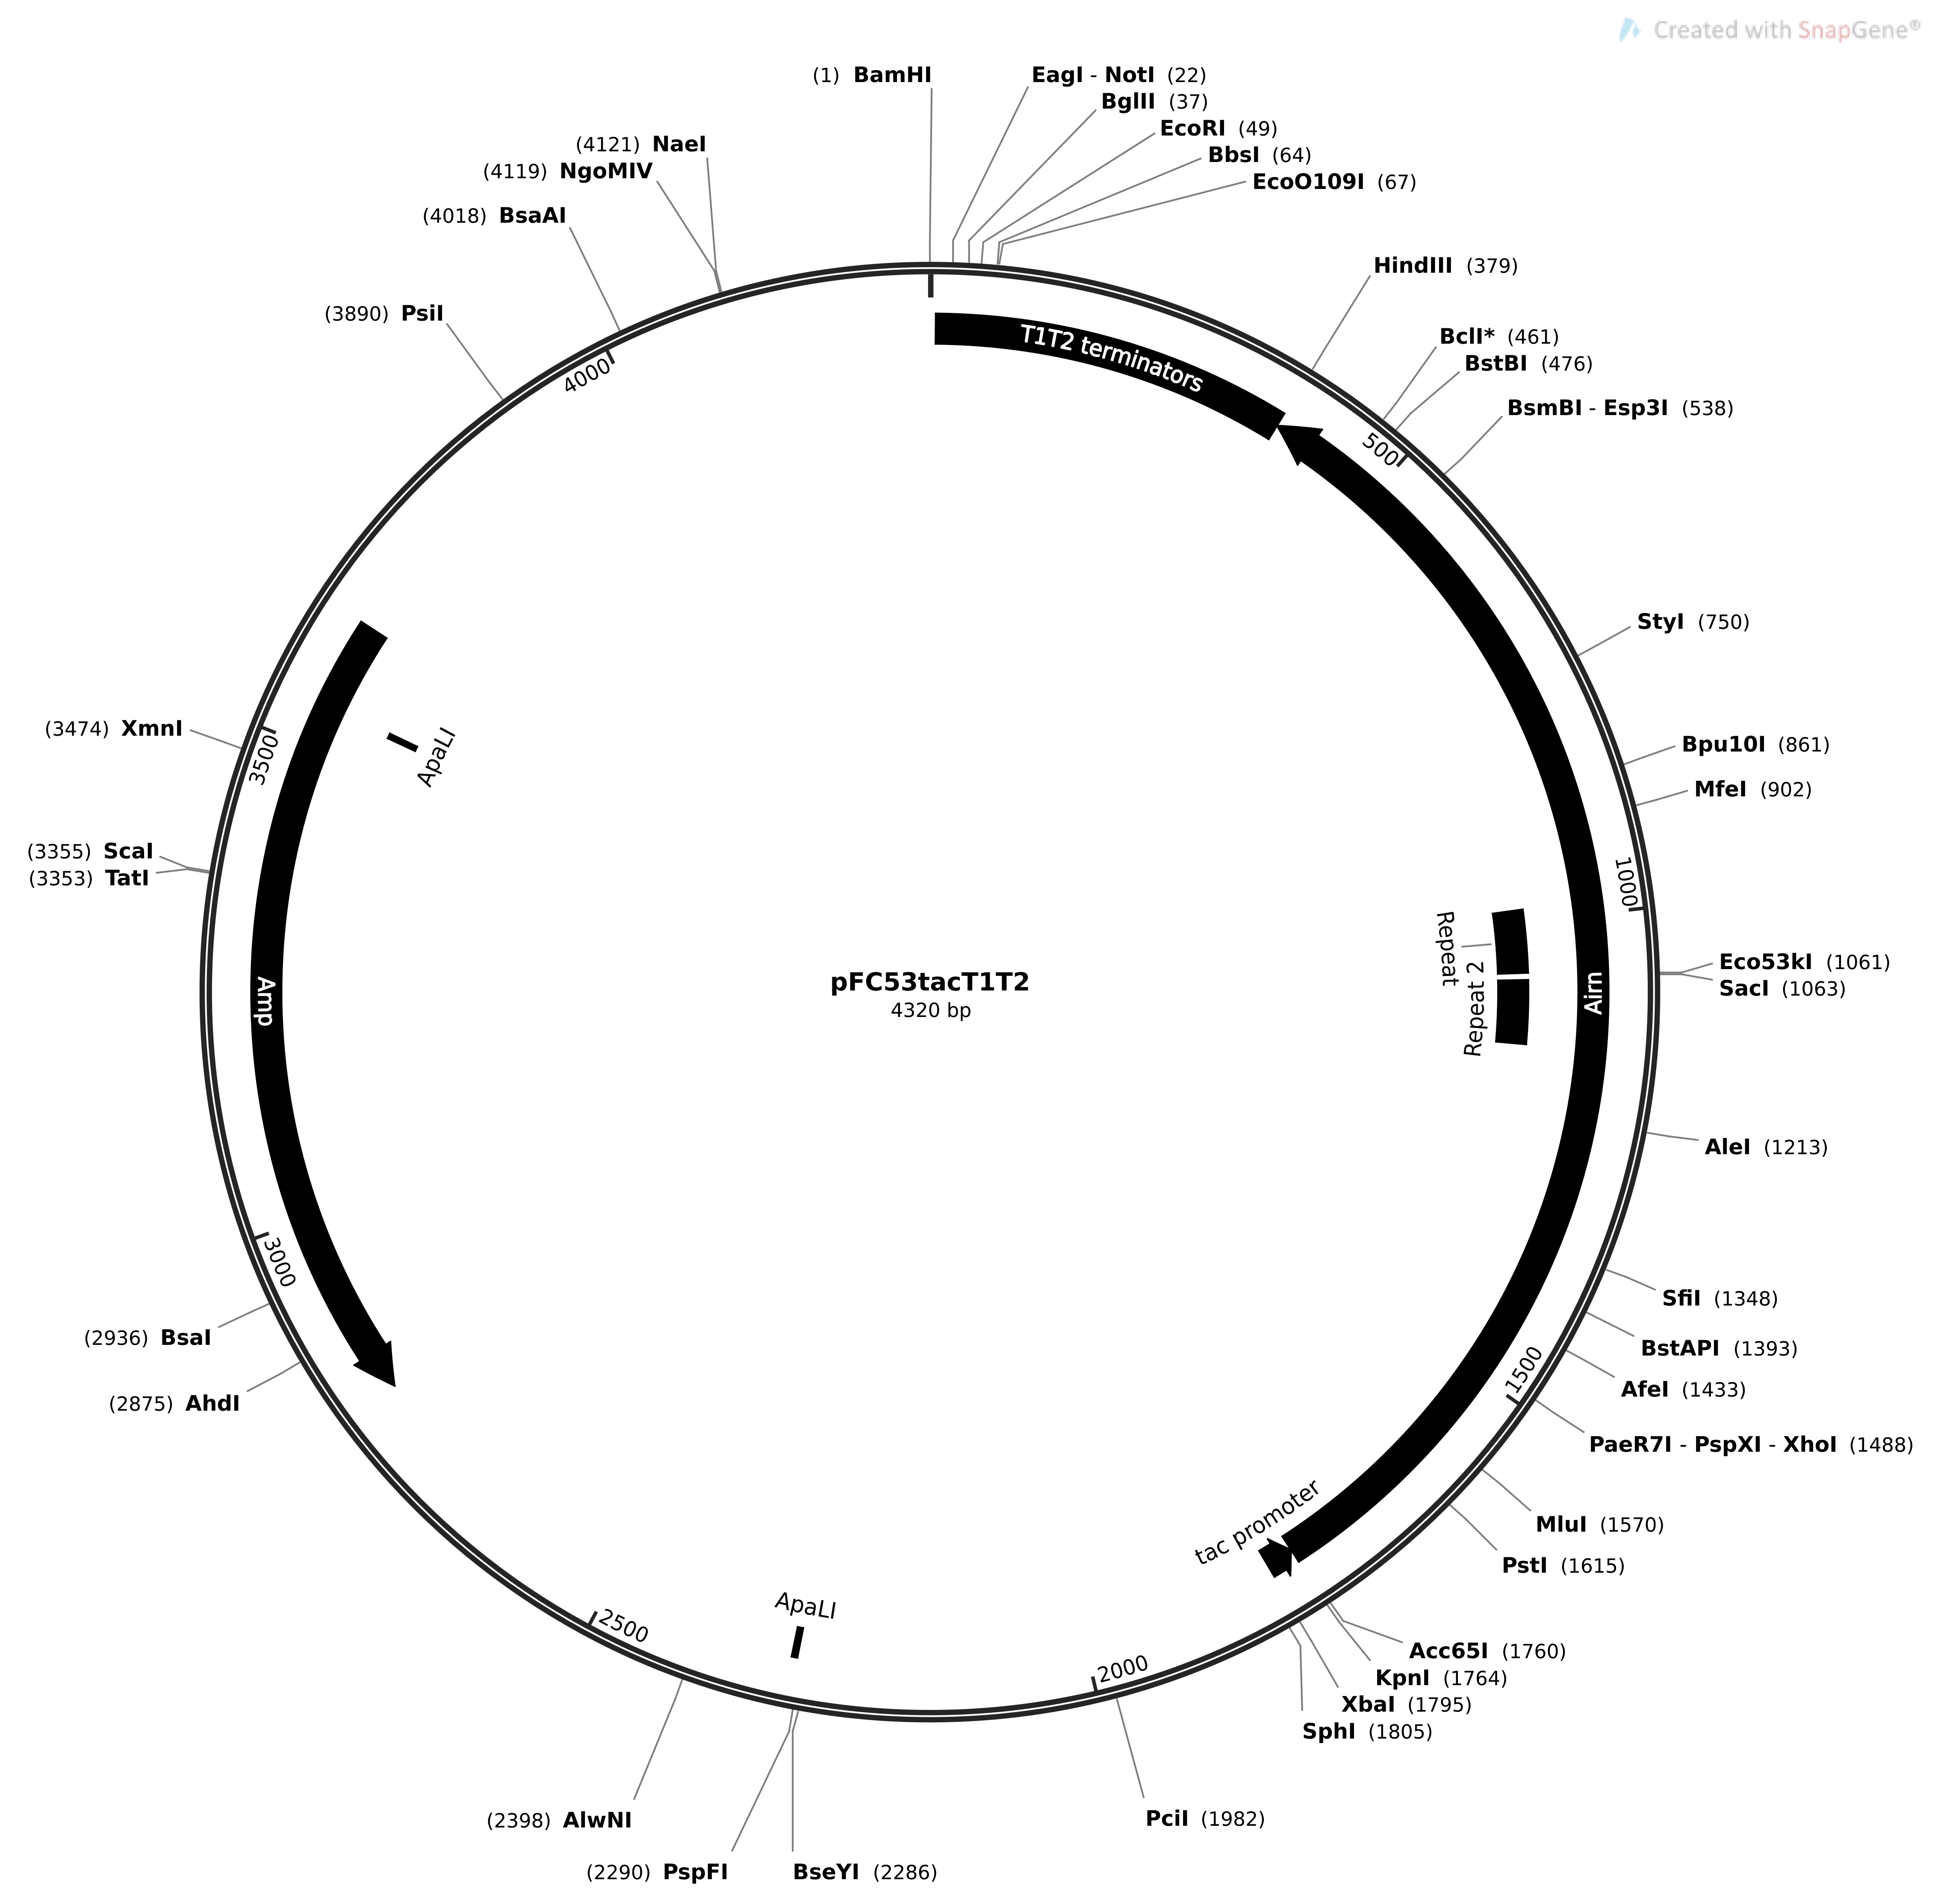
\includegraphics[width=12cm]{images/plasmid_maps/pFC53tacT1T2_Map.png}
	\centering
	\caption{Map of pFC53tacT1T2.}
	\label{fig:pFC53tacT1T2}
\end{figure}


\begin{figure}[H]
	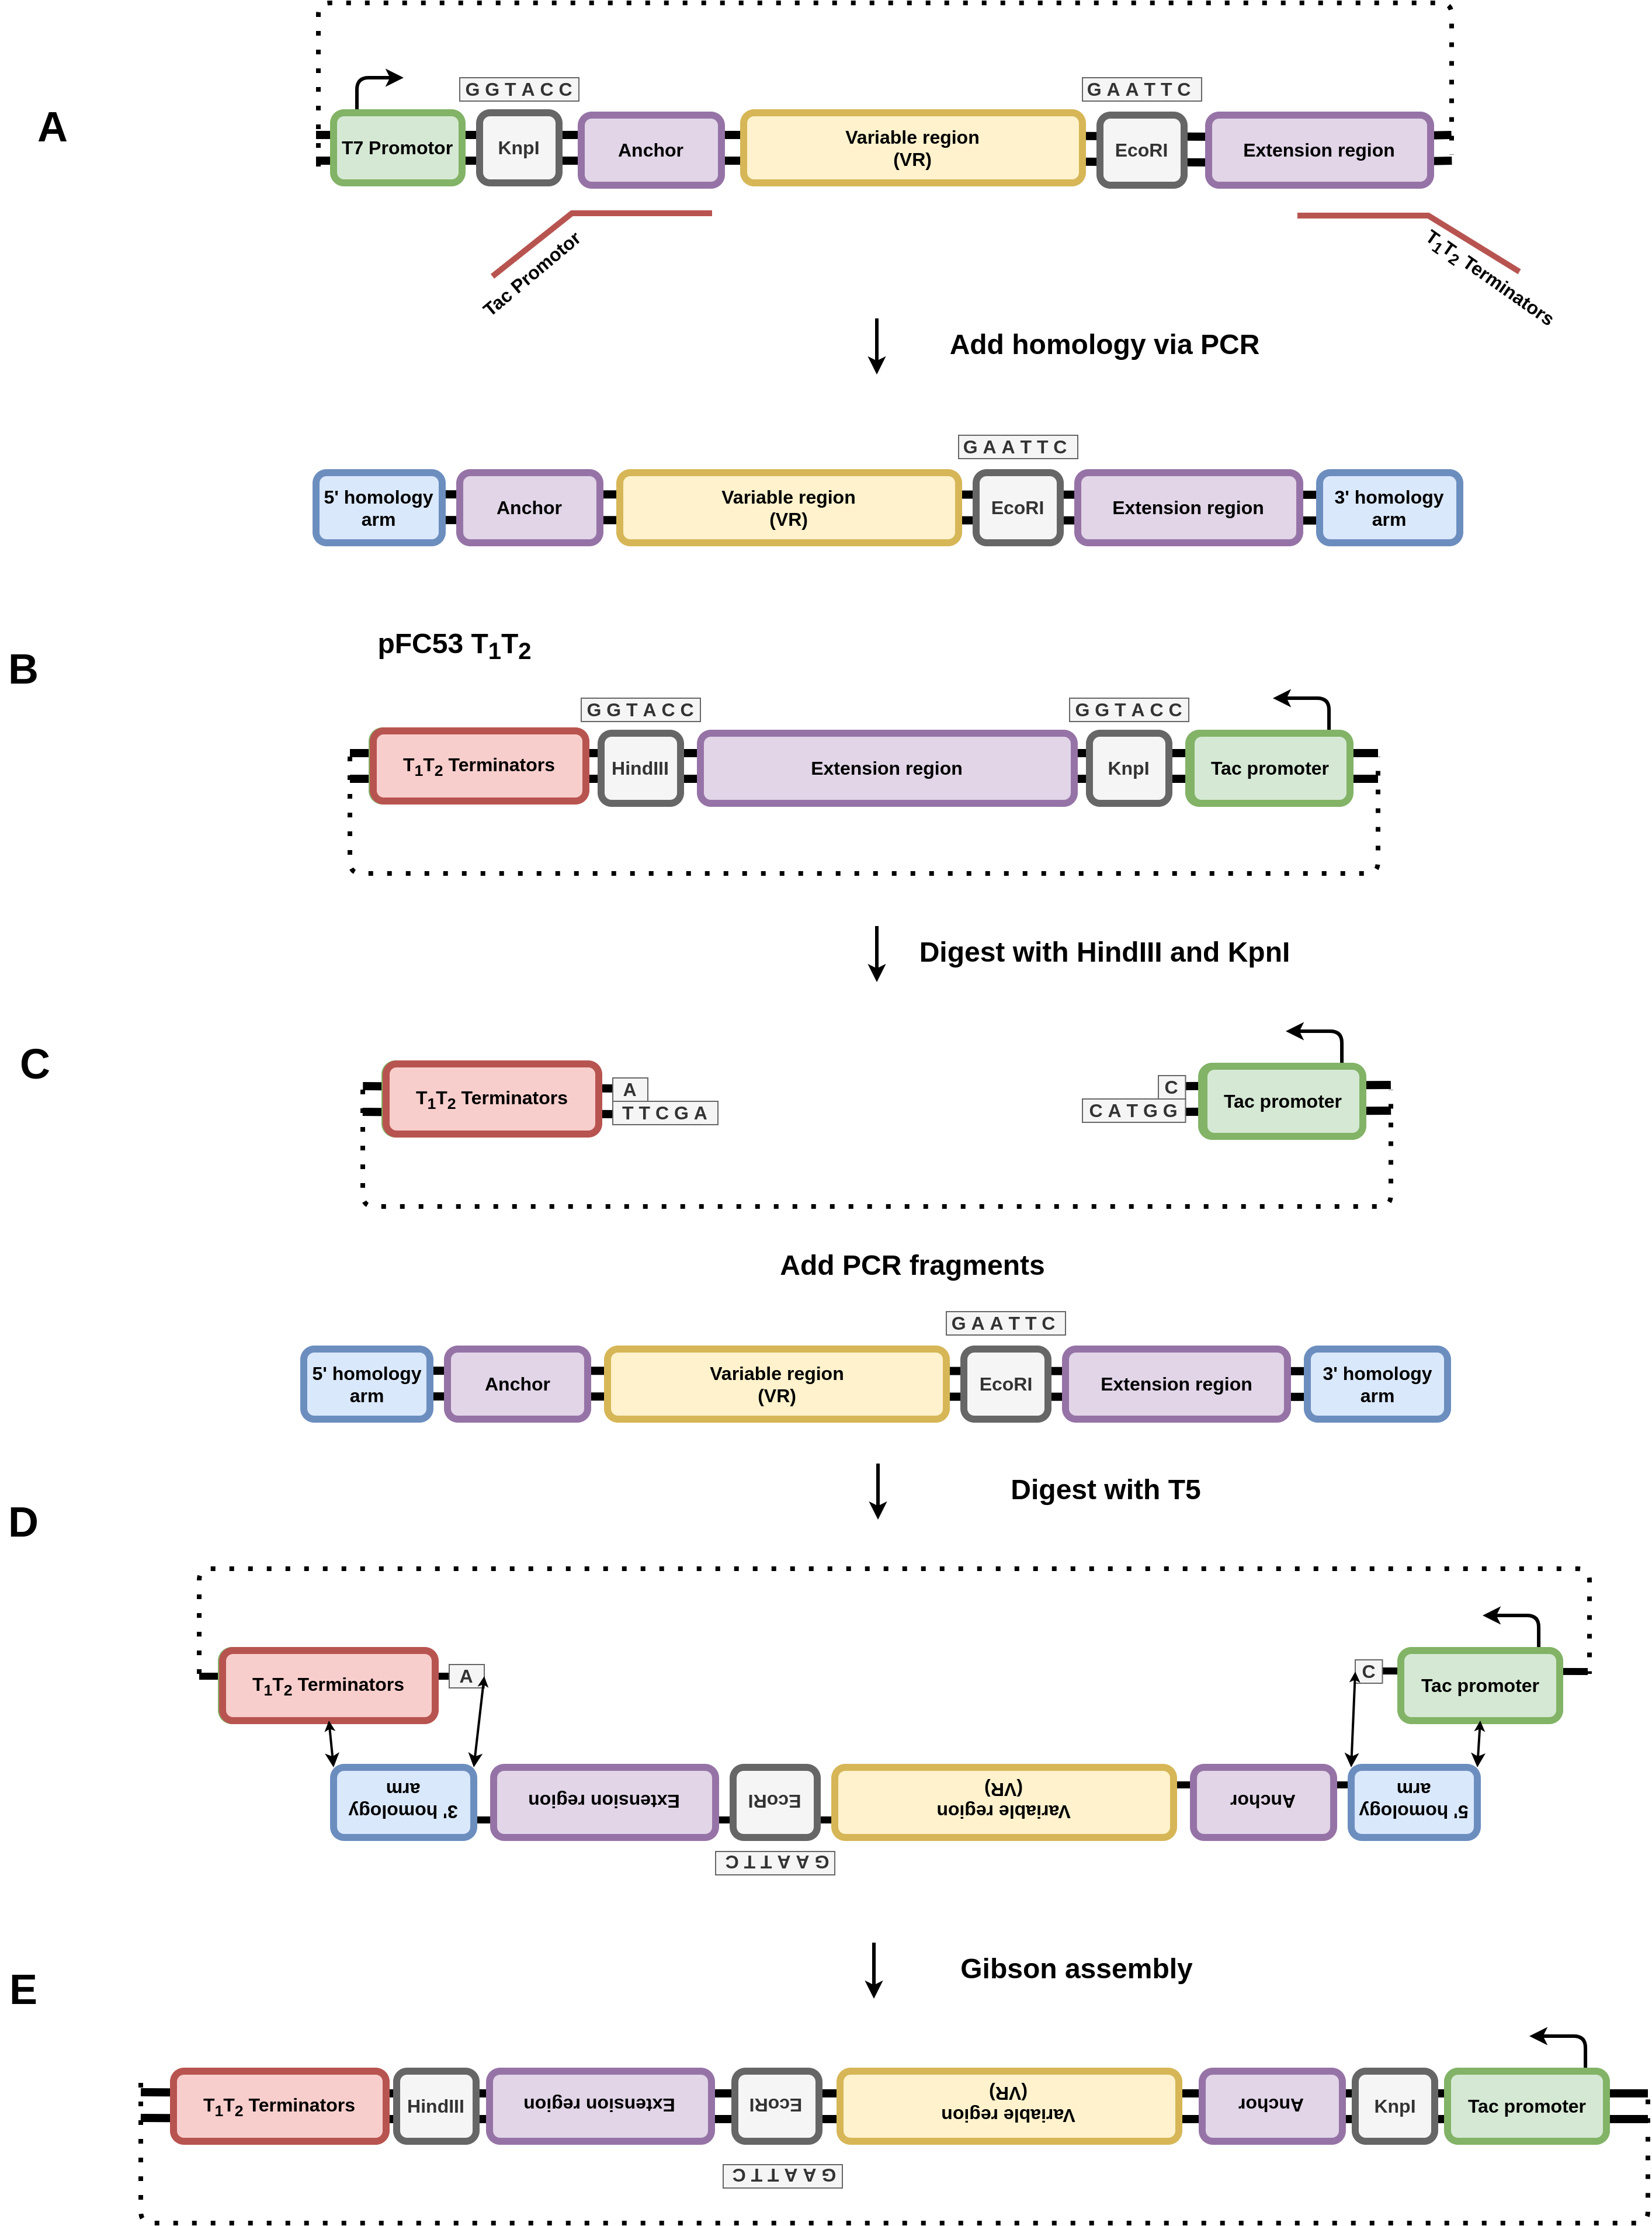
\includegraphics[width=15cm]{images/cloning_diagrams/construct_diagrams-Tac-initiation-series.png}
	\centering
	\caption{Diagram of pFC9 insertion series cloning strategy.}
\end{figure}

\subsection{Tac termination series constructs}


\begin{figure}[H]
	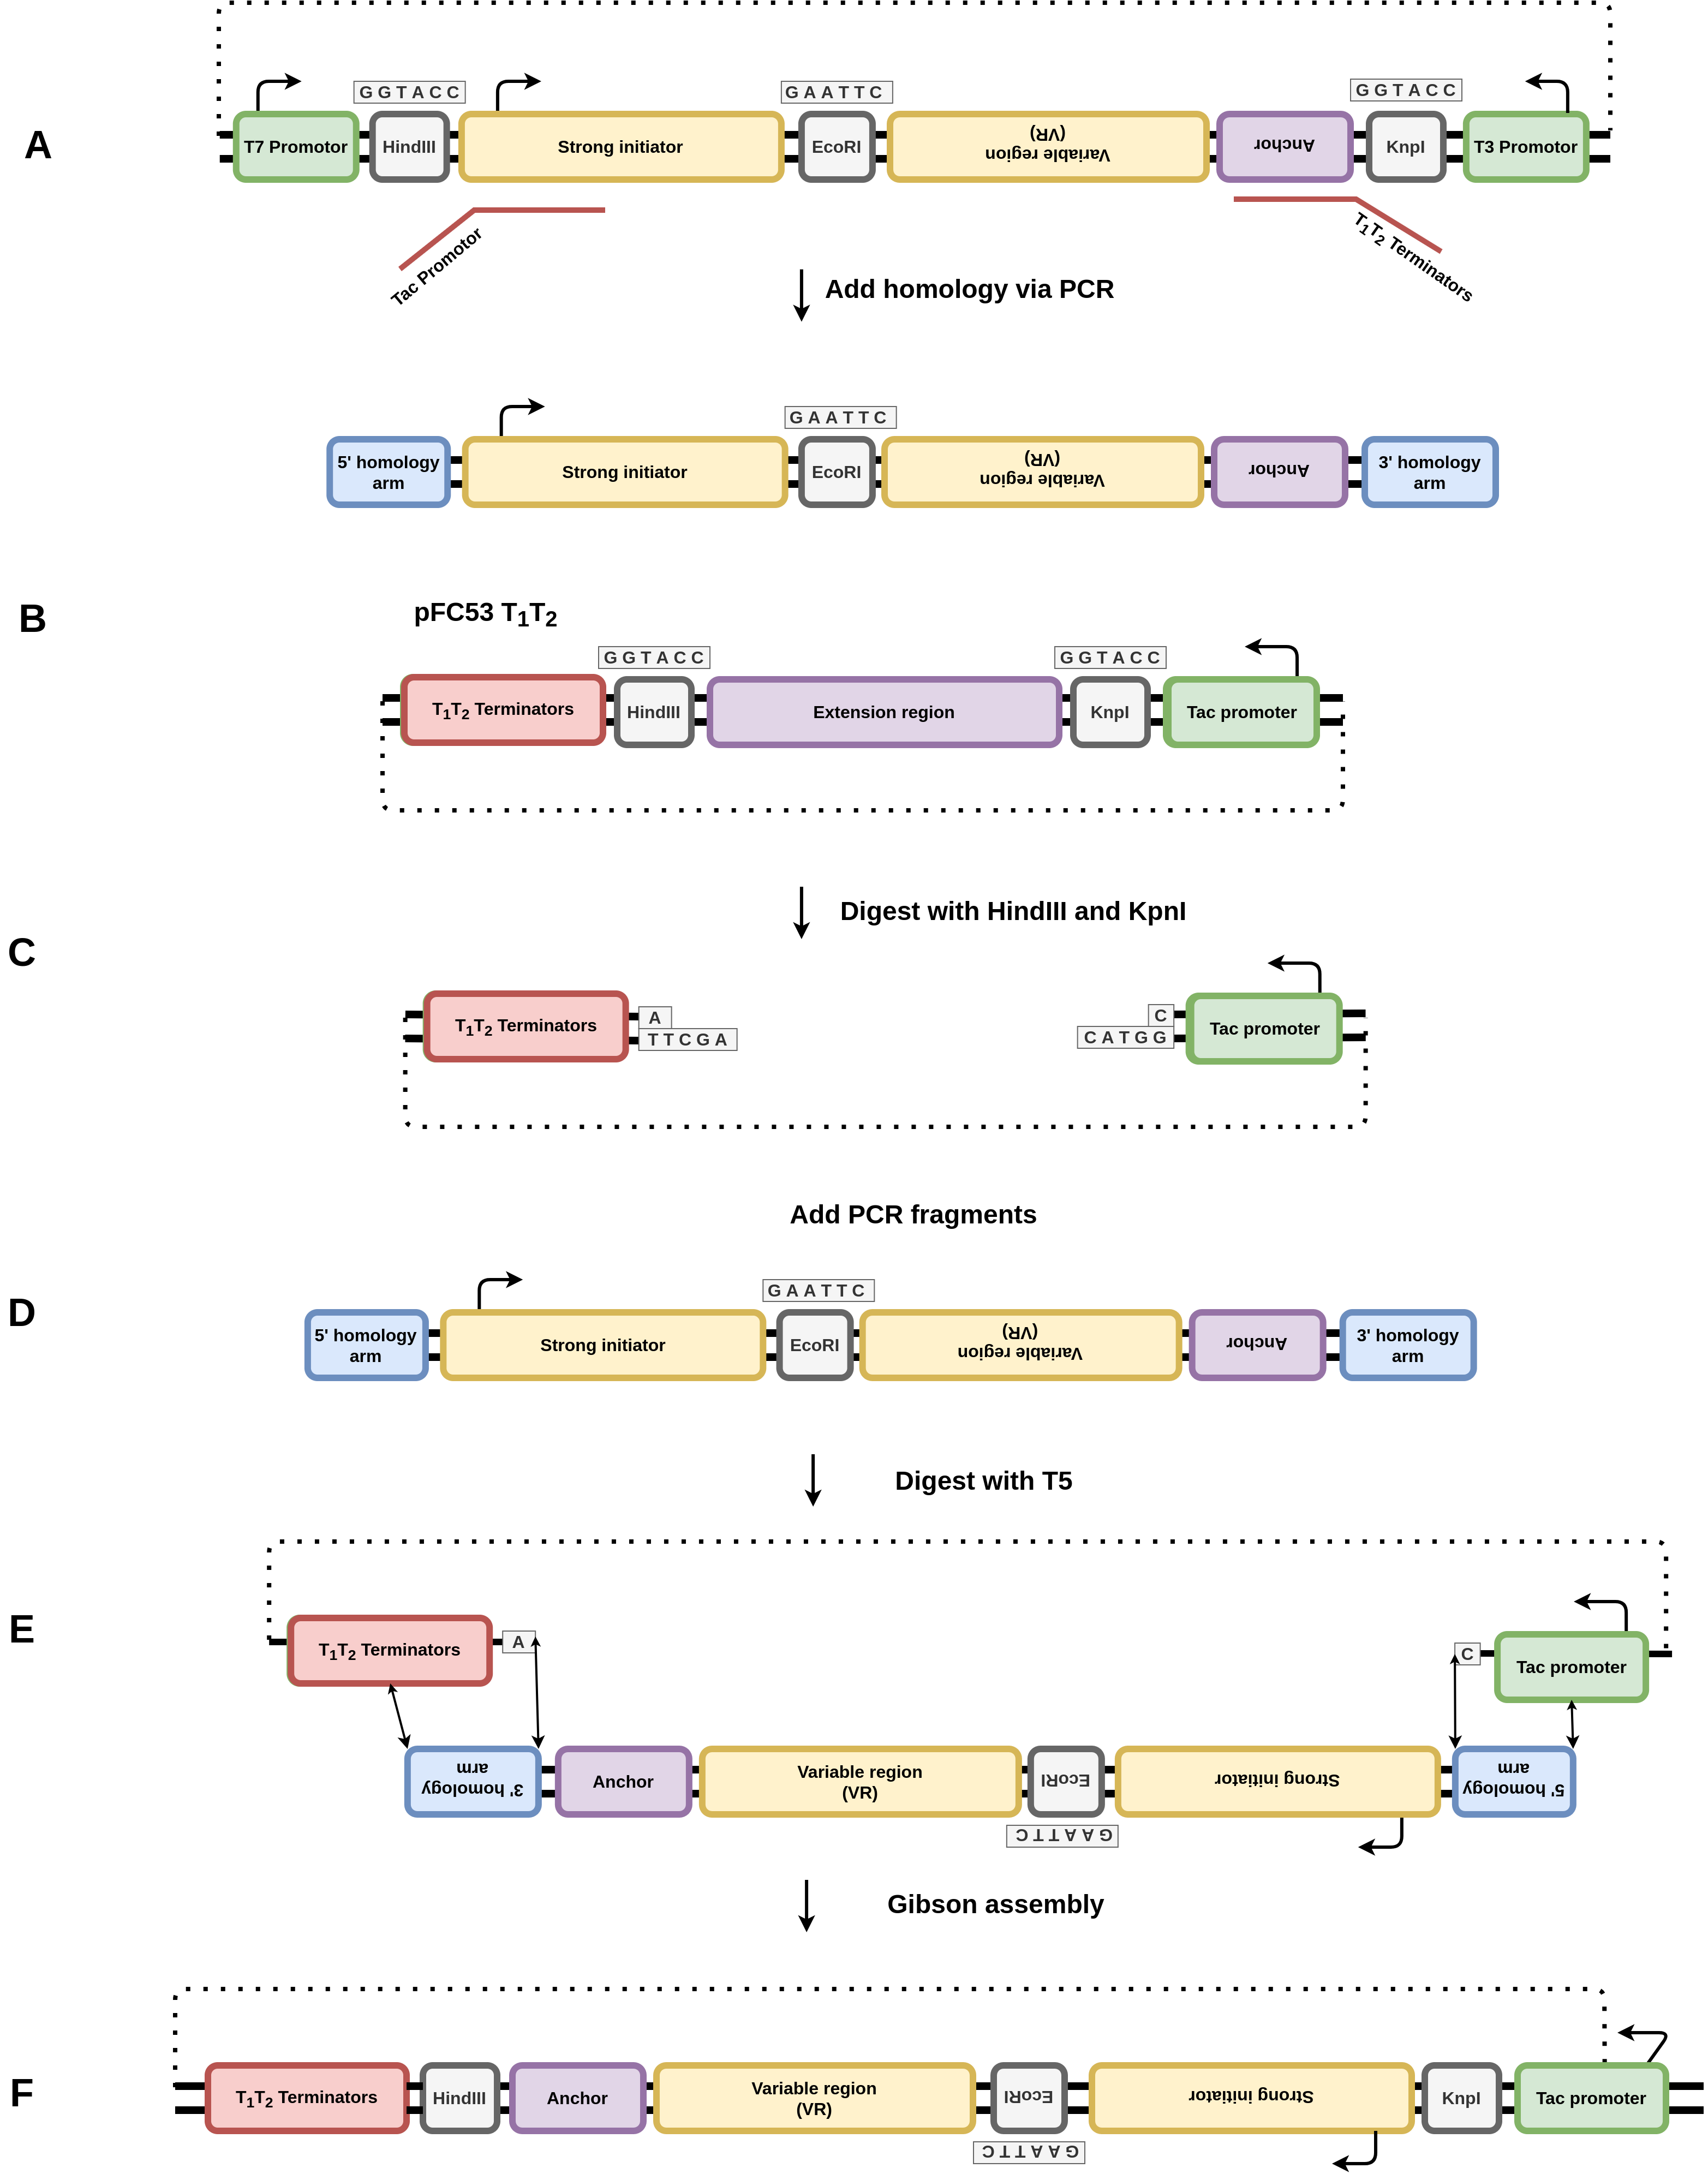
\includegraphics[width=15cm]{images/cloning_diagrams/construct_diagrams-Tac-termination-series.png}
	\centering
	\caption{Diagram of pFC9 insertion series cloning strategy.}
\end{figure}


\pagebreak

\bibliography{refs/refs.bib}

\end{document}
